\documentclass[a4paper,11pt,twoside]{article}
\usepackage[top=3cm,bottom=3cm,left=2cm,right=2cm]{geometry}
%\usepackage{multirow}
\usepackage{footnote}
\usepackage{amsbsy}
\usepackage{amsmath}
\usepackage{graphicx}
\usepackage{fancyhdr}
\usepackage{subfig}
\usepackage[T1]{fontenc} % important for having searchable underscores
\usepackage{bm}% bold math
\usepackage[sort&compress,numbers]{natbib}
%\setlength{\parindent}{0in}
%\setlength{\parskip}{0.05in}
\setlength{\parskip}{0.1in}

%%%%%%%%%%%%%%%%%%%%%%%%%%% REMOVE AT THE END %%%%%%%%%%%%%%%%%%%%%%%%%%%
\usepackage[usenames]{color} % colors
\usepackage{ulem} % allows \sout (strikeout). Can remove at the end (Ivo)
%\usepackage{soul} % allows \hl (highlight). Can remove at the end (Ivo)
\newcommand\tent[1]{\textcolor{red}{#1}}     % for tentative changes
\newcommand\tentbis{\color{red}}     % for tentative changes
%%%%%%%%%%%%%%%%%%%%%%%%%%% REMOVE AT THE END %%%%%%%%%%%%%%%%%%%%%%%%%%%
%\let\oldundercore=\_
%\def\_{\oldunderscore}

\usepackage{textcomp}

% set fancy headings

\pagestyle{fancy}
\lhead[{\it \thepage}]{{\bf\it {\tt wannier90}: Tutorial}}
\chead{}
\rhead[{\bf\it {\tt wannier90}: Tutorial}]{{\it \thepage}}
\renewcommand{\headrulewidth}{0.2pt}
\lfoot{}
\cfoot{}
\rfoot{}
\renewcommand{\footrulewidth}{0pt}
\setlength{\footskip}{0.25in}
\setlength{\parindent}{0in}

\title{\wannier: Tutorial}

\author{Version 3.0}

\date{27th February 2019}
%\date{\today}

%%% THIS SHOULD BE THE LAST PACKAGE TO BE LOADED!
%hidelinks to remove colored borders from links
%plainpages=false needed for the unnumbered pages
%breaklinks=true to allow to break long links (e.g. long titles) on
%more than one line
%bookmarksopen open the bookmarks in the adobe reader plugin
%bookmarksopenlevel decide the max level at which the bookmarks should
%be open
% pdfdisplaydoctitle=true to show the document title instead of the
% filename in the titlebar of adobereader
\usepackage[plainpages=false,breaklinks=true,pdfborder=0 0 0,pdfdisplaydoctitle=true,bookmarksopen=true,bookmarksopenlevel=0,pdftex,%
% Comment the following line if it makes problems (it requires a recent
% LaTeX distribution)
            hidelinks,
            pdftitle={Wannier90 Tutorial},
            pdfkeywords={wannier90;postw90;pwscf;tutorial;examples}]{hyperref}


\begin{document}
\newcommand{\wannier}{{\rm\texttt{wannier90}}}
\newcommand{\postw}{{\rm\texttt{postw90}}}
\newcommand{\bw}{{\rm\texttt{BoltzWann}}}
\newcommand{\pwscf}{\textsc{pwscf}}
\newcommand{\QE}{\textsc{quantum-espresso}}
\newcommand{\Mkb}{\mathbf{M}^{(\mathbf{k},\mathbf{b})}}
\newcommand{\Ak}{\mathbf{A}^{(\mathbf{k})}}
\newcommand{\Uk}{\mathbf{U}^{(\mathbf{k})}}

\newcommand\sectiontitle[1]{\section*{#1}\addcontentsline{toc}{section}{#1}}

\maketitle

\tableofcontents

\newpage


\sectiontitle{Preliminaries}
\label{sec:preliminaries}

Welcome to \wannier! The examples contained in this tutorial are
designed to help you become familiar with the procedure of generating,
analysing and using maximally-localised Wannier functions (MLWFs). As
a first step, install \wannier\ following the instructions in the {\tt
  README} file of the \wannier\ distribution.  For an introduction to
the theory underlying MLWFs, you are encouraged to refer to the brief
overview given in the \wannier\ User Guide~\cite{UserGuide}, to the
two seminal papers of Refs.~\cite{marzari-prb97,souza-prb01}, a recent
review article~\cite{marzari-rmp12} and to a
paper~\cite{mostofi-cpc08} describing \wannier.

The following additional programs may be installed in order to
visualise the output of \wannier\ (they are optional, not all of them
are necessary)
\begin{itemize}
\item {\tt gnuplot} is used to plot bandstructures. It is 
available for many operating systems and is often installed by default on
 Unix/Linux distributions\\
\url{http://www.gnuplot.info}
\item {\tt xmgrace} may also be used to plot bandstructures.\\
\url{http://plasma-gate.weizmann.ac.il/Grace}
\item {\tt XCrySDen} is used to visualise crystal structures, MLWFs,
  and Fermi surfaces. It is available for Unix/Linux, 
  Windows (using cygwin), and OSX. To correctly display 
files from \wannier, version 1.4 or later must be used.\\
\url{http://www.xcrysden.org}
\item {\tt vmd} can also be used to visualise crystal structures and
  MLWFs.\\
\url{http://www.ks.uiuc.edu/Research/vmd}
\item{\tt python} with the {\tt numpy} and {\tt matplotlib} modules
  is used in examples 17--19\\
  \url{http://www.python.org}\\
  \url{http://www.numpy.org}\\
  \url{http://matplotlib.org}
\end{itemize}

\sectiontitle{Parallel execution}
\label{sec:parallel}
{\tt postw90.x} and {\tt wannier90.x} can be run in parallel to speed up
the calculations, using the MPI libraries.

To enable the parallel version to be built, you must specify some
flags in the {\tt make.inc} file of {\tt wannier90} and {\tt postw90};
for further information, please refer to the {\tt README.install} file
in the top directory of the {\tt wannier90} distribution.

Then, to run e.g. with 8 processors, you typically need to run a
command similar to {\tt postw90} as follows:
\begin{verbatim}
mpirun -np 8 postw90.x seedname
\end{verbatim}
(the {\tt mpirun} command and its flags may differ depending on the
MPI libraries installed on your system: refer to your MPI manual and/or to
your system administrator for further information).



\sectiontitle{About this tutorial}

The first part of this tutorial comprises four examples taken from
Refs.~\cite{marzari-prb97,souza-prb01}: gallium arsenide, lead,
silicon and copper. All of the \wannier\ input files have been
provided.

The second part of the tutorial covers the generation of \wannier\
input files starting from a full electronic structure calculation. We
have provided input files for the \pwscf\ interface (\url{http://www.quantum-espresso.org}) to \wannier. 
Therefore, you
will need to install and compile elements of the {\tt
  quantum-espresso} package, namely {\tt pw.x} and {\tt
  pw2wannier90.x}, in order to run these
examples. Please visit \url{http://www.quantum-espresso.org} to download the
package, and for installation instructions. 
The tutorial examples work with \pwscf\ v5.1.x and v6.0.x. The exception are the examples on symmetry adapted Wannier functions which require v6.0.x together with the  
very latest version of {\tt pw2wannier90.f90}. This can be found in the directory {\tt pwscf/v6.0} in the wannier distribution. It should be moved to {\tt PP/src} in the \pwscf\ distribution and compiled using {\tt make pp}. Later versions v6.x.x should have the most up-to-date version 
 of pw2wannier90.f90 already included in the Quantum ESPRESSO  
 distribution. 


There are interfaces to a number of other electronic structure codes
including {\sc abinit} (\url{http://www.abinit.org}), {\sc fleur}
(\url{http://www.flapw.de}),  {\sc OpenMX} (\url{http://www.openmx-square.org/}), 
{\sc GPAW} (\url{https://wiki.fysik.dtu.dk/gpaw/}), {\sc VASP} (\url{http://www.vasp.at}), and
{\sc Wien2k} (\url{http://www.wien2k.at})

\sectiontitle{Contact us}

If you have any suggestions regarding ways in which this tutorial may
be improved, then send us an email.
% at {\tt developers@wannier.org}. 

For other questions, email the \wannier\ forum at {\tt
  wannier@quantum-espresso.org}.  Note that first you will need to
register in order to post emails. Emails from non-registered users are
deleted automatically. You can register by following the links at\\
\url{http://www.wannier.org/forum.html}.



\cleardoublepage

\sectiontitle{1: Gallium Arsenide -- MLWFs for the valence bands}

\begin{itemize}
\item{Outline: \it{Obtain and plot MLWFs for the four valence
    bands of GaAs.}} 
\item{Generation details: \it{From \pwscf, using norm-conserving
    pseudopotentials and a 2$\times$2$\times$2 k-point grid. Starting
    guess: four bond-centred Gaussians.}}
\item{Directory: {\tt examples/example1/}}
\item{Input Files}
\begin{itemize}
\item{ {\tt gaas.win}  {\it The master input file}}
\item{ {\tt gaas.mmn}  {\it The overlap matrices $\Mkb$}}
\item{ {\tt gaas.amn}  {\it Projection $\Ak$ of the Bloch states onto a set
    of trial localised orbitals}} 
\item{ {\tt UNK00001.1}  {\it The Bloch states in the real space unit
    cell. For plotting only.}} 
\end{itemize}
\end{itemize}

\begin{enumerate}
\item Run \wannier\ to minimise the MLWFs spread
{\tt
\begin{quote}
wannier90.x gaas
\end{quote} }
Inspect the output file {\tt gaas.wout}. The total spread converges to its
minimum value after just a few iterations. Note that the geometric centre of
each MLWF lies along a Ga-As bond, slightly closer to As
than Ga. Note also that the memory requirement for the minimisation of
the spread is very low as the MLWFs are defined at each
k-point by just the 4$\times$4 unitary matrices $\Uk$. 
\item Plot the MLWFs by adding the following keywords to
  the input file {\tt gaas.win} 
{\tt
\begin{quote}
wannier\_\-plot = true
\end{quote} } and re-running \wannier. To visualise the MLWFs we must
represent them explicitly on a real space grid (see
Ref.~\cite{UserGuide}). As a consequence, plotting the MLWFs is slower
and uses more memory than the minimisation of the spread. The four
files that are created ({\tt gaas\_00001.xsf}, etc.) can be viewed
using {\tt XCrySDen},\footnote{Once {\tt XCrySDen} starts, click on
  {\tt Tools} $\rightarrow$ {\tt Data Grid} in order to specify an
  isosurface value to plot.} e.g., {\tt
\begin{quote}
xcrysden \texttt{-{}-}xsf gaas\_00001.xsf
\end{quote} }

For large systems, plotting the MLWFs may be time consuming
and require a lot of memory. Use the keyword {\tt wannier\_plot\_list}
to plot a subset of the MLWFs. E.g., to plot the
1st and 3rd MLWFs use 
{\tt
\begin{quote}
wannier\_plot\_list = 1 3
\end{quote} }
The MLWFs are plotted in a supercell of the unit cell. The
size of this supercell is set through the keyword {\tt
  wannier\_plot\_supercell}. The default value is 2 (corresponding to a
supercell with eight times the unit cell volume). We recommend not using
values great than 3 as the memory and computational cost scales
cubically with supercell size.  

Plot the 3rd MLWFs in a supercell of size 3. Choose a low
value for the isosurface (say 0.5). Can you explain what you see? 

{\it Hint:} For a finite k-point mesh, the MLWFs are in fact
periodic and the period is related to the spacing of the k-point mesh. For
mesh with $n$ divisions in the $i^{\mathrm{th}}$ direction in the
Brillouin zone, the MLWFs ``live'' in a supercell $n$ times the
unit cell. 
\end{enumerate}


%\cleardoublepage



\sectiontitle{2: Lead -- Wannier-interpolated Fermi surface}

\begin{itemize}
\item{Outline: \it{Obtain MLWFs for the four lowest states
    in lead. Use Wannier interpolation to plot the Fermi surface.}}
\item{Generation Details: \it{From \pwscf, using norm-conserving
    pseudopotentials and a 4$\times$4$\times$4 k-point grid. Starting
    guess: atom-centred sp$^3$ hybrid orbitals}} 
\item{Directory: {\tt examples/example2/}}
\item{Input Files}
\begin{itemize}
\item{ {\tt lead.win}  {\it The master input file}}
\item{ {\tt lead.mmn}  {\it The overlap matrices $\Mkb$}}
\item{ {\tt lead.amn}  {\it Projection $\Ak$ of the Bloch states onto a set
    of trial localised orbitals}} 
\item{ {\tt lead.eig}  {\it The Bloch eigenvalues at each k-point. For
    interpolation only}} 
\end{itemize}

\end{itemize}

The four lowest valence bands in lead are separated in energy from the
higher conduction states (see Fig.~\ref{fig:pb-bnd}). The MLWFs of
these states have partial occupancy. MLWFs describing only the occupied
states would be poorly localised.

\begin{enumerate}
\item Run \wannier\ to minimise the MLWFs spread
{\tt
\begin{quote}
wannier90.x lead
\end{quote} }
Inspect the output file {\tt lead.wout}.
\item Use Wannier interpolation to generate the Fermi surface of
  lead. Rather than re-running the whole calculation we can use the
  unitary transformations obtained in the first calculation and
  restart from the plotting routine. Add the following keywords to the
  {\tt lead.win} file: {\tt
\begin{quote}
restart = plot

fermi\_energy = 5.2676

fermi\_surface\_plot = true
\end{quote} } and re-run \wannier. The value of the Fermi energy
(5.2676\,eV) was obtained from the initial first principles
calculation. \wannier\ calculates the band energies, through 

interpolation, on a dense mesh of k-points in the Brillouin zone. The
density of this grid is controlled by the keyword {\tt
  fermi\_surface\_num\_points}. The default value is 50 (i.e., 50$^3$
points).  The Fermi surface file {\tt lead.bxsf} can be viewed using
{\tt XCrySDen}, e.g., 
%
{\tt
\begin{quote}
xcrysden \texttt{-{}-}bxsf lead.bxsf
\end{quote} }
\end{enumerate}

\begin{figure}[h]
\begin{center}
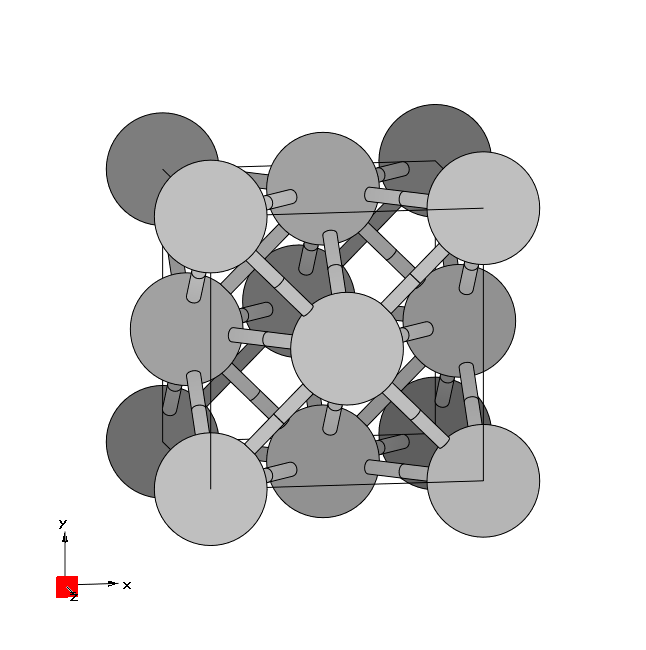
\includegraphics{lead}
\caption{Bandstructure of lead showing the position of the Fermi
  level. Only the lowest four bands are included in the calculation.} 
\label{fig:pb-bnd}
\end{center}
\end{figure}

%\cleardoublepage


\sectiontitle{3: Silicon -- Disentangled MLWFs}

\begin{itemize}
\item{Outline: \it{Obtain disentangled MLWFs for the valence and
      low-lying conduction states of Si. Plot the interpolated
      bandstructure}}
\item{Generation Details: \it{From \pwscf, using norm-conserving
    pseudopotentials and a 4$\times$4$\times$4 k-point grid. Starting
    guess: atom-centred sp$^3$ hybrid orbitals}} 
\item{Directory: {\tt examples/example3/}}
\item{Input Files}
\begin{itemize}
\item{ {\tt silicon.win}  {\it The master input file}}
\item{ {\tt silicon.mmn}  {\it The overlap matrices $\Mkb$}}
\item{ {\tt silicon.amn}  {\it Projection $\Ak$ of the Bloch states onto a
    set of trial localised orbitals}} 
\item{ {\tt silicon.eig}  {\it The Bloch eigenvalues at each k-point}}
\end{itemize}
\end{itemize}
The valence and lower conduction states can be represented by MLWFs
with $sp^3$-like symmetry. The lower conduction states are not 
separated from the higher states by an energy gap. In order to form
localised WF, we use the disentanglement procedure
introduced in Ref.~\cite{souza-prb01}. The position of the inner and outer
energy windows are shown in Fig.~\ref{fig:si.bnd}. 
\begin{enumerate}
\item Run \wannier.
{\tt
\begin{quote}
wannier90.x silicon
\end{quote} }
Inspect the output file {\tt silicon.wout}. The minimisation of the
spread occurs in a two-step procedure~\cite{souza-prb01}. First, we minimise
$\Omega_{\rm I}$ -- this is the extraction of the optimal subspace in
the disentanglement procedure. Then, we minimise $\Omega_{\rm D} +
\Omega_{{\rm OD}}$.

\item Plot the energy bands by adding the following
  commands to the input file {\tt silicon.win} {\tt
\begin{quote}
restart = plot

bands\_plot = true
\end{quote} }
and re-running \wannier. The files {\tt silicon\_band.dat} and {\tt
  silicon\_band.gnu} are created. 
To plot the bandstructure using gnuplot
\smallskip
{\tt
\begin{quote}
myshell> gnuplot

gnuplot> load `silicon\_band.gnu'
\end{quote} }
The k-point path for the bandstructure interpolation is set in the {\tt
  kpoint\_path} block. Try plotting along different paths. 
\end{enumerate}

\begin{figure}[h]
\begin{center}
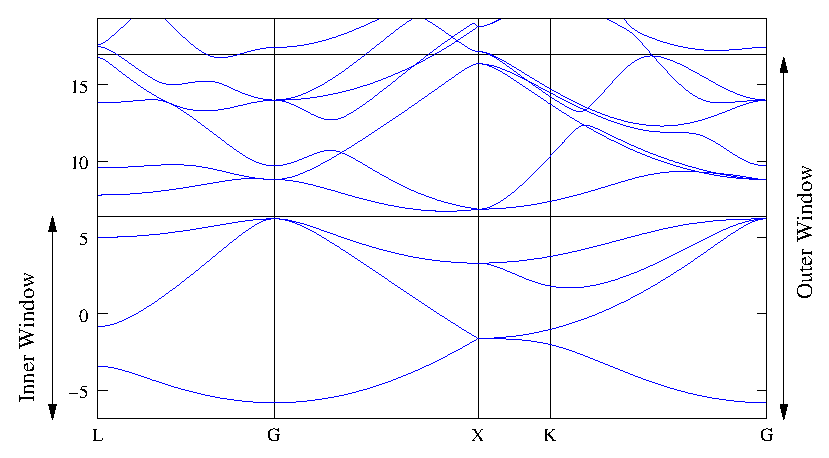
\includegraphics{si}
\caption{Bandstructure of silicon showing the position of the outer
  and inner energy windows.} 
\label{fig:si.bnd}
\end{center}
\end{figure}

%\cleardoublepage


\sectiontitle{4: Copper -- Fermi surface, orbital character of energy
  bands}

\begin{itemize}
\item{Outline: \it{Obtain MLWFs to describe the states around the
    Fermi-level in copper}} 
\item{Generation Details: \it{From \pwscf, using ultrasoft
    pseudopotentials~\cite{vanderbilt-prb90} and a
    4$\times$4$\times$4 k-point grid. Starting guess: five 
    atom-centred d orbitals, and two s orbitals centred on one of each
    of the two tetrahedral interstices.}}
\item{Directory: {\tt examples/example4/}}
\item{Input Files}
\begin{itemize}
\item{ {\tt copper.win}  {\it The master input file}}
\item{ {\tt copper.mmn}  {\it The overlap matrices $\Mkb$}}
\item{ {\tt copper.amn}  {\it Projection $\Ak$ of the Bloch states onto a
    set of trial localised orbitals}} 
\item{ {\tt copper.eig}  {\it The Bloch eigenvalues at each k-point}}
\end{itemize}

\end{itemize}

\begin{enumerate}
\item Run \wannier\ to minimise the MLWFs spread
{\tt
\begin{quote}
wannier90.x copper
\end{quote} }
Inspect the output file {\tt copper.wout}. 

\item Plot the Fermi surface, it should look familiar! The Fermi
  energy is at 12.2103\,eV. 

\item Plot the interpolated bandstructure. A suitable path in k-space is
\smallskip
{\tt
\begin{quote}
begin kpoint\_path

G 0.00  0.00  0.00    X 0.50  0.50  0.00

X 0.50  0.50  0.00    W 0.50  0.75  0.25

W 0.50  0.75  0.25    L 0.00  0.50  0.00

L 0.00  0.50  0.00    G 0.00  0.00  0.00

G 0.00  0.00  0.00    K 0.00  0.50 -0.50
 
end kpoint\_path
\end{quote} }
\item Plot the contribution of the interstitial WF to the
  bandstructure. Add the following keyword to {\tt copper.win}
\smallskip
{\tt
\begin{quote}
bands\_plot\_project = 6,7
\end{quote} } The resulting file {\tt copper\_band\_proj.gnu} can be
opened with gnuplot. Red lines correspond to a large contribution from
the interstitial WF (blue line are a small contribution; ie a large
$d$ contribution).


\end{enumerate}




Investigate the effect of the outer and inner energy window on the
interpolated bands. 



\begin{figure}[h]
\begin{center}
\includegraphics{cu}
\caption{Bandstructure of copper showing the position of the outer
  and inner energy windows.} 
\label{fig:cu-bnd}
\end{center}
\end{figure}

\clearpage

\sectiontitle{Examples Using the {\sc pwscf} Interface}
\label{sec:using pwscf}

The \pwscf\ plane-wave, density-functional theory code, which is
available as part of the \QE\ distribution (\url{http://www.quantum-espresso.org}), is fully interfaced to \wannier\ via the
{\tt pw2wannier90} post-processing code that is also available as part
of \QE. The latest version of {\tt pw2wannier90} is included as part of 
the \wannier\ distribution. Please see the {\tt pwscf} directory for 
instructions on how to incorporate it into \pwscf. 

Note that both the {\tt PWSCF} executable {\tt pw.x} {\it and} {\tt
  pw2wannier90.x} can be run in parallel, which for large calculations
can reduce the computation time very significantly.  This requires
compiling the code in its parallel version, using the MPI
libraries. Refer to the \QE\ package for the documentation on how to
do so.  Note that, unless you specify {\tt wf\_collect=.true.} in your
{\tt pw.x} input file, you must run {\tt pw2wannier90} with the same
number of processors as {\tt pw.x}.

Moreover we remind here that both the \wannier\ executable and {\tt postw90.x} can be run in
parallel. In this case any number of processors can be used,
independently of the number used for {\tt pw.x} and {\tt
  pw2wannier90.x}.

%\cleardoublepage

\sectiontitle{5: Diamond -- MLWFs for the valence bands}
\begin{itemize}
\item{Outline: \it{Obtain MLWFs for the valence bands of diamond}}
\item{Directory: {\tt examples/example5/}}
\item{Input Files}
\begin{itemize}
\item{ {\tt diamond.scf}  {\it The \pwscf\ input file for ground state
    calculation}} 
\item{ {\tt diamond.nscf}  {\it The \pwscf\ input file to obtain Bloch
    states on a uniform grid}} 
\item{ {\tt diamond.pw2wan}  {\it The input file for {\tt pw2wannier90}}}
\item{ {\tt diamond.win}  {\it The {\tt wannier90} input file}}
\end{itemize}
\end{itemize}

\begin{enumerate}
\item Run \pwscf\ to obtain the ground state of diamond\\
{\tt pw.x < diamond.scf > scf.out}

\item Run \pwscf\ to obtain the Bloch states on a uniform k-point grid\\
{\tt pw.x < diamond.nscf > nscf.out}

\item Run \wannier\ to generate a list of the required overlaps (written
  into the {\tt diamond.nnkp} file).\\ 
{\tt wannier90.x -pp diamond}

\item Run {\tt pw2wannier90} to compute the overlap between Bloch
  states and the projections for the starting guess (written in the
  {\tt diamond.mmn} and {\tt diamond.amn} files).\\  
{\tt pw2wannier90.x < diamond.pw2wan > pw2wan.out}

\item Run \wannier\ to compute the MLWFs.\\
{\tt wannier90.x diamond}
\end{enumerate}

%\cleardoublepage

\sectiontitle{6: Copper -- Fermi surface}

\begin{itemize}
\item{Outline: \it{Obtain MLWFs to describe the states around the
    Fermi-level in copper}}
\item{Directory: {\tt examples/example6/}}
\item{Input Files}
\begin{itemize}
\item{ {\tt copper.scf}  {\it The \pwscf\ input file for ground state
    calculation}} 
\item{ {\tt copper.nscf}  {\it The \pwscf\ input file to obtain Bloch states
    on a uniform grid}} 
\item{ {\tt copper.pw2wan}  {\it Input file for {\tt pw2wannier90}}}
\item{ {\tt copper.win}  {\it The {\tt wannier90} input file}}
\end{itemize}

\end{itemize}

\begin{enumerate}
\item Run \pwscf\ to obtain the ground state of copper\\
{\tt pw.x < copper.scf > scf.out}

\item Run \pwscf\ to obtain the Bloch states on a uniform k-point grid\\
{\tt pw.x < copper.nscf > nscf.out}

\item Run \wannier\ to generate a list of the required overlaps (written
  into the {\tt copper.nnkp} file).\\ 
{\tt wannier90.x -pp copper}

\item Run {\tt pw2wannier90} to compute the overlap between Bloch
  states and the projections for the starting guess (written in the
  {\tt copper.mmn} and {\tt copper.amn} files).\\  
{\tt pw2wannier90.x < copper.pw2wan > pw2wan.out}

\item Run \wannier\ to compute the MLWFs.\\
{\tt wannier90.x copper}
\end{enumerate}

Inspect the output file {\tt copper.wout}. 

\begin{enumerate}
\item Use Wannier interpolation to obtain the Fermi surface of
  copper. Rather than re-running the whole calculation we can use the
  unitary transformations obtained in the first calculation and restart
  from the plotting routine. Add the following keywords to the {\tt
    copper.win} file:
{\tt
\begin{quote}
restart = plot

fermi\_energy = [insert your value here] 

fermi\_surface\_plot = true
\end{quote} } and re-run \wannier. The value of the Fermi energy can
be obtained from the initial first principles calculation. \wannier\
calculates the band energies, through Wannier interpolation, on a
dense mesh of k-points in the Brillouin zone. The density of this grid
is controlled by the keyword {\tt fermi\_surface\_num\_points}. The
default value is 50 (i.e., 50$^3$ points).  The Fermi surface file
{\tt copper.bxsf} can be viewed using {\tt XCrySDen}, e.g.,
%
{\tt
\begin{quote}
xcrysden \texttt{-{}-}bxsf copper.bxsf
\end{quote} }


\item Plot the interpolated bandstructure. A suitable path in k-space is
\smallskip
{\tt
\begin{quote}
begin kpoint\_path

G 0.00  0.00  0.00    X 0.50  0.50  0.00

X 0.50  0.50  0.00    W 0.50  0.75  0.25

W 0.50  0.75  0.25    L 0.00  0.50  0.00

L 0.00  0.50  0.00    G 0.00  0.00  0.00

G 0.00  0.00  0.00    K 0.00  0.50 -0.50
 
end kpoint\_path
\end{quote} }
\end{enumerate}

\subsection*{Further ideas}
\begin{itemize}
\item Compare the Wannier interpolated bandstructure with the full
  \pwscf\ bandstructure. Obtain MLWFs using a denser k-point grid.
To plot the bandstructure you can use the \pwscf\ tool {\tt bands.x} or the small FORTRAN program available at \url{http://www.tcm.phy.cam.ac.uk/~jry20/bands.html}.
\item Investigate the effects of the outer and inner energy windows on
  the interpolated bands. 
\item Instead of extracting a subspace of seven states, we could
  extract a nine dimensional space (i.e., with $s$, $p$ and $d$
  character). Examine this case and compare the interpolated
  bandstructures.
\end{itemize}

%\begin{figure}[h]
%\begin{center}
%\includegraphics{cu}
%\caption{Band Structure of Copper showing the position of the outer
%  and inner energy windows.}
%\label{fig:cu-bnd}
%\end{center}
%\end{figure}

%\cleardoublepage

\sectiontitle{7: Silane (SiH$_4$) -- Molecular MLWFs using
  $\Gamma$-point sampling}
\begin{itemize}
\item{Outline: \it{Obtain MLWFs for the occupied states of molecular
    silane. $\Gamma$-point sampling}} 
\item{Directory: {\tt examples/example7/}}
\item{Input Files}
\begin{itemize}
\item{ {\tt silane.scf}  {\it The \pwscf\ input file for ground state
    calculation}} 
\item{ {\tt silane.nscf}  {\it The \pwscf\ input file to obtain Bloch states
    on a uniform grid}} 
\item{ {\tt silane.pw2wan}  {\it Input file for {\tt pw2wannier90}}}
\item{ {\tt silane.win}  {\it The {\tt wannier90} input file}}
\end{itemize}
\end{itemize}

\begin{enumerate}
\item Run \pwscf\ to obtain the ground state of silane\\
{\tt pw.x < silane.scf > scf.out}

\item Run \pwscf\ to obtain the Bloch states on a uniform k-point grid\\
{\tt pw.x < silane.nscf > nscf.out}

\item Run \wannier\ to generate a list of the required overlaps (written
  into the {\tt silane.nnkp} file).\\ 
{\tt wannier90.x -pp silane}

\item Run {\tt pw2wannier90} to compute the overlap between Bloch
  states and the projections for the starting guess (written in the
  {\tt silane.mmn} and {\tt silane.amn} files).\\  
{\tt pw2wannier90.x < silane.pw2wan > pw2wan.out}

\item Run \wannier\ to compute the MLWFs.\\
{\tt wannier90.x silane}
\end{enumerate}

%\cleardoublepage

\sectiontitle{8: Iron -- Spin-polarized WFs, DOS, projected WFs versus MLWFs}
\begin{itemize}
\item{Outline: \it{Generate both maximally-localized and projected
      Wannier functions for ferromagnetic bcc Fe. Calculate the total
      and orbital-projected density of states by Wannier
      interpolation.}}
\item{Directory: {\tt examples/example8/}}
\item{Input Files}
\begin{itemize}
\item{ {\tt iron.scf} {\it The \pwscf\ input file for the
      spin-polarized ground state calculation}}
\item{ {\tt iron.nscf}  {\it The \pwscf\ input file to obtain Bloch states
    on a uniform grid}} 
\item{ {\tt iron\_\{up,down\}.pw2wan}  {\it Input files for {\tt pw2wannier90}}} 
\item{ {\tt iron\_\{up,down\}.win} {\it Input files for {\tt wannier90} and {\tt
          postw90}}}
\end{itemize}
\item{Note that in a spin-polarized calculation the spin-up and
    spin-down MLWFs are computed separately. (The more general case of
    spinor WFs will be treated in Example~17.)}
\end{itemize}

\begin{enumerate}
\item Run \pwscf\ to obtain the ferromagnetic ground state of bcc Fe\\
{\tt pw.x < iron.scf > scf.out}

\item Run \pwscf\ to obtain the Bloch states on a uniform k-point grid\\
{\tt pw.x < iron.nscf > nscf.out}

\item Run \wannier\ to generate a list of the required overlaps (written
  into the {\tt .nnkp} files).\\
{\tt wannier90.x -pp iron\_up}\\
{\tt wannier90.x -pp iron\_dn}

\item Run {\tt pw2wannier90} to compute the overlap between Bloch
  states and the projections for the starting guess (written in the
  {\tt .mmn} and {\tt .amn} files).\\
  {\tt pw2wannier90.x < iron\_up.pw2wan > pw2wan\_up.out}\\
  {\tt pw2wannier90.x < iron\_dn.pw2wan > pw2wan\_dn.out}

\item Run \wannier\ to compute the MLWFs.\\
{\tt wannier90.x iron\_up}\\
{\tt wannier90.x iron\_dn}

\end{enumerate}

\subsection*{Density of states}

To compute the DOS using a $25\times 25 \times 25$ $k$-point grid add
to the two {\tt .win} files
%
{\tt
\begin{quote}
dos = true

dos\_kmesh = 25
\end{quote}
}
%
run {\tt postw90},
%
{\tt
\begin{quote}
postw90.x iron\_up

postw90.x iron\_dn
\end{quote}
}
%
and plot the DOS with {\tt gnuplot},
%
{\tt
\begin{quote}
myshell> gnuplot

gnuplot> plot `iron\_up\_dos.dat' u (-\$2):(\$1-12.6256) w l,`iron\_dn\_dos.dat' u 2:(\$1-12.6256) w l

\end{quote} 
}
%
Energies are referred to the Fermi level (12.6256~eV, from {\tt
  scf.out}).  Note the exchange splitting between the up-spin and
down-spin DOS. Check the convergence by repeating the DOS calculations
with more $k$-points.

\subsection*{Projected versus maximally-localized Wannier functions}

In the calculations above we chose $s$, $p$, and $d$-type trial
orbitals in the {\tt .win} files,
%
{\tt
\begin{quote}
Fe:s;p;d
\end{quote}
}
%
Let us analyze the evolution of the WFs during the gauge-selection
step. Open one of the {\tt .wout} files and search for ``{\tt Initial
  state}''; those are the {\it projected} WFs. As expected they are
atom-centred, with spreads organized in three groups, 1+3+5: one $s$,
three $p$, and five $d$.  Now look at the final state towards the end
of the file.  The Wannier spreads have re-organized in two groups,
6+3; moreover, the six more diffuse WFs are off-centred: the initial
atomic-like orbitals hybridized with one another, becoming more
localized in the process. It is instructive to visualize the
final-state MLWFs using {\tt XCrySDen}, following Example~1. For more
details, see Sec.~IV.B of Ref.~\cite{wang-prb06}.

Let us plot the evolution of the spread functional~$\Omega$,
%
{\tt
\begin{quote}
myshell> grep SPRD iron\_up.wout > sprd\_up

myshell> gnuplot

gnuplot> plot `sprd\_up' u 6  w l
\end{quote}
}

\begin{figure}[h]
\begin{center}
\scalebox{0.35}{\includegraphics{Fe-spread}}
\caption{Evolution of the Wannier spread $\Omega$ of the minority
  (spin-up) bands of bcc Fe during the iterative minimization of
  $\widetilde{\Omega}$, starting from $s$, $p$, and $d$-type trial
  orbitals.}
\label{fig:Fe-sprd}
\end{center}
\end{figure}


The first plateau corresponds to atom-centred WFs of separate $s$,
$p$, and $d$ character, and the sharp drop signals the onset of the
hybridization. With hindsight, we can redo steps~4 and~5 more
efficiently using trial orbitals with the same character as the final
MLWFs,
%
{\tt
\begin{quote}
Fe:sp3d2;dxy;dxz,dyz
\end{quote}
}
%
With this choice the minimization converges much more rapidly.

Any reasonable set of localized WFs spanning the states of interest
can be used to compute physical quantities (they are
``gauge-invariant''). Let us recompute the DOS using, instead of
MLWFs, the WFs obtained by projecting onto $s$, $p$, and $d$-type
trial orbitals, without further iterative minimization of the spread
functional. This can be done by setting
%
{\tt
\begin{quote}
num\_iter = 0
\end{quote}
}
%
But note that we still need to do disentanglement!
Recalculate the DOS to confirm that it is almost identical to the one
obtained earlier using the hybridized set of MLWFs. Visualize the
projected WFs using {\tt XCrySDen}, to see that they retain the pure
orbital character of the individual trial orbitals.


\subsection*{Orbital-projected DOS and exchange splitting}

With projected WFs the total DOS can be separated into $s$, $p$ and
$d$ contributions, in a similar way to the orbital decomposition of
the energy bands in Example~4.
  
In order to obtain the partial DOS projected onto the $p$-type WFs,
add to the {\tt .win} files
%
{\tt
\begin{quote}
dos\_project = 2,3,4
\end{quote}
}
%
and re-run {\tt postw90}. Plot the projected DOS for both up- and
down-spin bands. Repeat for the $s$ and $d$ projections. 

Projected WFs can also be used to quantify more precisely the exchange
splitting between majority and minority states. Re-run {\tt wannier90}
after setting {\tt dos=false} and adding to the {\tt .win} files
%
{\tt
\begin{quote}
write\_hr\_diag = true
\end{quote}
}
%
This instructs {\tt wannier90} to print in the output file the on-site
energies $\langle {\bf 0}n\vert H\vert {\bf 0}n\rangle$. The
difference between corresponding values in {\tt iron\_up.wout} and in
{\tt iron\_dn.wout} gives the exchange splittings for the individual
orbitals. Compare their magnitudes with the splittings displayed by
the orbital-projected DOS plots.  In agreement with the Stoner
criterion, the largest exchange splittings occur for the localized
$d$-states, which contribute most of the density of states at the
Fermi level.


%\cleardoublepage


\sectiontitle{9: Cubic BaTiO$_3$}
\begin{itemize}
\item{Outline: \it{Obtain MLWFs for a perovskite}}
\item{Directory: {\tt examples/example9/}}
\item{Input Files}
\begin{itemize}
\item{ {\tt batio3.scf}  {\it The \pwscf\ input file for ground state
    calculation}} 
\item{ {\tt batio3.nscf}  {\it The \pwscf\ input file to obtain Bloch states
    on a uniform grid}} 
\item{ {\tt batio3.pw2wan}  {\it Input file for {\tt pw2wannier90}}}
\item{ {\tt  batio3.win}  {\it The {\tt wannier90} input file}}
\end{itemize}
\end{itemize}

 To start with, we are going to obtain MLWFs for the oxygen 2p
  states. From the bandstructure~\cite{marzari-arxiv98}, these form an isolated
  group of bands. We use the \wannier\ keyword {\tt exclude\_bands} to
  remove all but the 2p bands from the calculation of the overlap
  and projection matrices (we don't have to do this, but it saves time).

\begin{enumerate}
\item Run \pwscf\ to obtain the ground state of BaTiO$_3$\\
{\tt pw.x < BaTiO3.scf > scf.out}

\item Run \pwscf\ to obtain the Bloch states on a uniform k-point grid\\
{\tt pw.x < BaTiO3.nscf > nscf.out}

\item Run \wannier\ to generate a list of the required overlaps (written
  into the {\tt BaTiO3.nnkp} file).\\ 
{\tt wannier90.x -pp BaTiO3}

\item Run {\tt pw2wannier90} to compute the overlap between Bloch
  states and the projections for the starting guess (written in the
  {\tt BaTiO3.mmn} and {\tt BaTiO3.amn} files).\\  
{\tt pw2wannier90.x < BaTiO3.pw2wan > pw2wan.out}

\item Run \wannier\ to compute the MLWFs.\\
{\tt wannier90.x BaTiO3}
\end{enumerate}

Inspect the output file {\tt BaTiO3.wout}. 

Plot the second MLWF, as described in Section~1, by adding the
following keywords to the input file {\tt BaTiO3.win}
{\tt
\begin{quote}
wannier\_plot = true\\
restart = plot\\
wannier\_plot\_list = 2\\
wannier\_plot\_supercell = 3
\end{quote} }
and re-running \wannier. Visualise it using {\tt XCrySDen},
{\tt
\begin{quote}
xcrysden \texttt{-{}-}xsf BaTiO3\_00002.xsf
\end{quote} }

We can now simulate the ferroelectric phase by displacing the Ti
  atom. Change its position to 
{\tt
\begin{quote}
Ti 0.505 0.5 0.5
\end{quote}
}
and regenerate the MLWFs (i.e., compute the ground-state charge
density and Bloch states using \pwscf, etc.) and look at the change in
the second MLWF.

\subsection*{Further ideas}
\begin{itemize}
\item Look at MLWFs for other groups of bands. What happens if you form
  MLWFs for the whole valence manifold?

\item Following Ref.~\cite{marzari-arxiv98}, compute the Born effective charges from the
  change in Wannier centres under an atomic displacement. 
\end{itemize}

%\cleardoublepage

\sectiontitle{10: Graphite}
\begin{itemize}
\item{Outline: \it{Obtain MLWFs for graphite (AB, Bernal)}}
\item{Directory: {\tt examples/example10/}}
\item{Input Files}
\begin{itemize}
\item{ {\tt graphite.scf}  {\it The \pwscf\ input file for ground
    state calculation}} 
\item{ {\tt graphite.nscf}  {\it The \pwscf\ input file to obtain Bloch
    states on a uniform grid}} 
\item{ {\tt graphite.pw2wan}  {\it Input file for {\tt pw2wannier90}}}
\item{ {\tt graphite.win}  {\it The {\tt wannier90} input file}}
\end{itemize}
\end{itemize}

\begin{enumerate}
\item Run \pwscf\ to obtain the ground state of graphite\\
{\tt pw.x < graphite.scf > scf.out}

\item Run \pwscf\ to obtain the Bloch states on a uniform k-point grid\\
{\tt pw.x < graphite.nscf > nscf.out}

\item Run \wannier\ to generate a list of the required overlaps (written
  into the {\tt graphite.nnkp} file).\\ 
{\tt wannier90.x -pp graphite}

\item Run {\tt pw2wannier90} to compute the overlap between Bloch
  states and the projections for the starting guess (written in the
  {\tt graphite.mmn} and {\tt graphite.amn} files).\\  
{\tt pw2wannier90.x < graphite.pw2wan > pw2wan.out}

\item Run \wannier\ to compute the MLWFs.\\
{\tt wannier90.x graphite}
\end{enumerate}


%\cleardoublepage


\sectiontitle{11: Silicon -- Valence and low-lying conduction states}
\subsection*{Valence States}
\begin{itemize}
\item{Outline: \it{Obtain MLWFs for the valence bands of silicon.}}
\item{Directory: {\tt examples/example11/}}
\item{Input Files}
\begin{itemize}
\item{ {\tt silicon.scf}  {\it The \pwscf\ input file for ground state
    calculation}} 
\item{ {\tt silicon.nscf}  {\it The \pwscf\ input file to obtain Bloch
    states on a uniform grid}} 
\item{ {\tt silicon.pw2wan}  {\it Input file for {\tt pw2wannier90}}}
\item{ {\tt silicon.win}  {\it The {\tt wannier90} input file}}
\end{itemize}

\end{itemize}

\begin{enumerate}
\item Run \pwscf\ to obtain the ground state of silicon\\
{\tt pw.x < silicon.scf > scf.out}

\item Run \pwscf\ to obtain the Bloch states on a uniform k-point
  grid. Note that we request the lower 4 (valence) bands\\ 
{\tt pw.x < silicon.nscf > nscf.out}

\item Run \wannier\ to generate a list of the required overlaps (written
  into the {\tt silicon.nnkp} file).\\
{\tt wannier90.x -pp silicon}

\item Run {\tt pw2wannier90} to compute the overlap between Bloch
  states and the projections for the starting guess (written in the
  {\tt silicon.mmn} and {\tt  silicon.amn} files).\\
{\tt pw2wannier90.x < silicon.pw2wan > pw2wan.out}

\item Run \wannier\ to compute the MLWFs.\\
{\tt wannier90.x silicon}

\end{enumerate}

Inspect the output file {\tt silicon.wout}. The total spread converges to its
minimum value after just a few iterations. Note that the geometric centre of
each MLWF lies at the centre of the Si-Si bond.
Note also that the memory requirement for the minimisation of
the spread is very low as the MLWFs are defined 
by just the 4$\times$4 unitary matrices $\Uk$. 

Plot the MLWFs by adding the following keywords to the input file {\tt
  silicon.win} 
{\tt
\begin{quote}
wannier\_plot = true
\end{quote} }
and re-running \wannier. Visualise them using {\tt XCrySDen}, e.g.,
{\tt
\begin{quote}
xcrysden \texttt{-{}-}xsf silicon\_00001.xsf
\end{quote} }

\subsection*{Valence + Conduction States}

\begin{itemize}
\item{Outline: \it{Obtain MLWFs for the valence and low-lying
      conduction-band states of Si. Plot the interpolated
      bandstructure. Apply a scissors correction to the conduction
      bands.}}
\item{Input Files}
\begin{itemize}
\item{ {\tt silicon.scf}  {\it The \pwscf\ input file for ground state
    calculation}} 
\item{ {\tt silicon.nscf}  {\it The \pwscf\ input file to obtain Bloch
    states on a uniform grid}} 
\item{ {\tt silicon.pw2wan}  {\it Input file for {\tt pw2wannier90}}}
\item{ {\tt silicon.win}  {\it The {\tt wannier90} input file}}
\end{itemize}
\end{itemize}
The valence and lower conduction states can be represented by MLWFs
with $sp^3$-like symmetry. The lower conduction states are not
separated by an energy gap from the higher states. In order to form
localised WF we use the disentanglement procedure introduced in
Ref.~\cite{souza-prb01}. The position of the inner and outer energy
windows are shown in Fig.~\ref{fig:si.bnd}.
\begin{enumerate}
\item Modify the input file and run \pwscf\ and \wannier.\\
Inspect the output file {\tt silicon.wout}. The minimisation of the
spread occurs in a two-step procedure. First, we minimise $\Omega_{\rm
  I}$ -- this is the extraction of the optimal subspace in the 
disentanglement procedure. Then, we minimise $\Omega_{\rm
  O}+\Omega_{{\rm OD}}$.

\item Plot the bandstructure by adding the following commands to the
 input file {\tt silicon.win}
{\tt
\begin{quote}
restart = plot

bands\_plot = true
\end{quote} }
and re-running \wannier. The files {\tt silicon\_band.dat} and {\tt
  silicon\_band.gnu} are created. To plot the bandstructure using
  gnuplot \smallskip
{\tt
\begin{quote}
myshell> gnuplot

gnuplot> load `silicon\_band.gnu'
\end{quote} }
The k-point path for the bandstructure interpolation is set in the {\tt
  kpoint\_path} block. Try plotting along different paths. 

%\item Shift the conduction bands upwards in energy by
%    0.65~eV. This {\it ad-hoc} ``scissors correction'' is applied to
%    the Hamiltonian in the Wannier basis using the instructions
%
%{\tt
%\begin{quote}
%num\_valence\_bands = 4
%
%scissors\_shift = 0.65
%\end{quote} }
%
%Plot together the original and scissors-corrected bands.

\end{enumerate}

\subsection*{Further ideas}

\begin{itemize}
\item Compare the Wannier-interpolated bandstructure with the full
  \pwscf\ bandstructure. Recompute the MLWFs using a finer $k$-point
  grid (e.g., 6$\times$6$\times$6 or 8$\times$8$\times$8) and note how
  the accuracy of the interpolation increases~\cite{yates-prb07}.
\item Compute four MLWFs spanning the low-lying conduction states (see
  Ref.~\cite{souza-prb01}).
\end{itemize}

%\begin{figure}[h]
%\begin{center}
%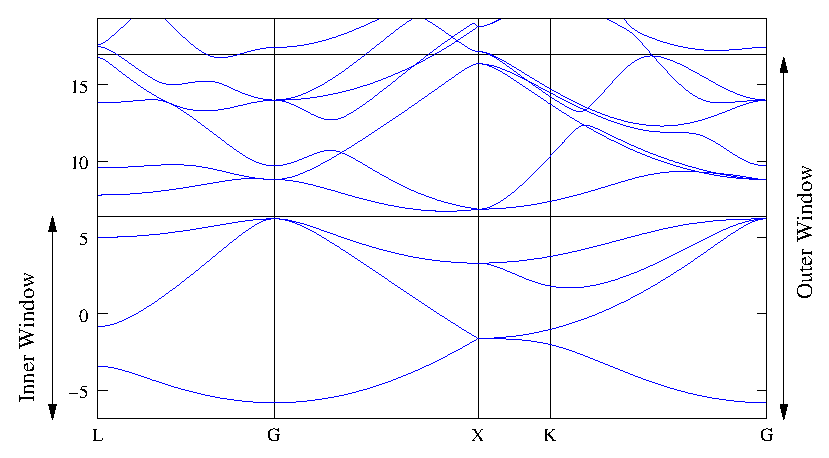
\includegraphics{si}
%\caption{Band Structure of Silicon showing the position of the outer
%and inner energy windows.}
%\label{fig:si.bnd}
%\end{center}
%\end{figure}

%\cleardoublepage


\sectiontitle{12: Benzene  -- Valence and low-lying conduction states}
\subsection*{Valence States}
\begin{itemize}
\item{Outline: \it{Obtain MLWFs for the valence states of benzene}}
\item{Directory: {\tt examples/example12/}}
\item{Input Files}
\begin{itemize}
\item{ {\tt benzene.scf}  {\it The \pwscf\ input file for ground state
    calculation}} 
\item{ {\tt benzene.pw2wan}  {\it Input file for {\tt pw2wannier90}}}
\item{ {\tt benzene.win}  {\it The {\tt wannier90} input file}}
\end{itemize}

\end{itemize}

\begin{enumerate}
\item Run \pwscf\ to obtain the ground state of benzene\\
{\tt pw.x < benzene.scf > scf.out}

\item Run \wannier\ to generate a list of the required overlaps (written
  into the {\tt benzene.nnkp} file).\\
{\tt wannier90.x -pp benzene}

\item Run {\tt pw2wannier90} to compute the overlap between Bloch
  states and the projections for the starting guess (written in the
  {\tt benzene.mmn} and {\tt  benzene.amn} files).\\
{\tt pw2wannier90.x < benzene.pw2wan > pw2wan.out}

\item Run \wannier\ to compute the MLWFs.\\
{\tt wannier90.x benzene}

\end{enumerate}

Inspect the output file {\tt benzene.wout}. The total spread converges
to its minimum value after just a few iterations. 

Plot the MLWFs by adding the following keywords to the input file {\tt
  benzene.win} 
{\tt
\begin{quote}
restart               = plot\\
wannier\_plot         = true\\
wannier\_plot\_format = cube\\
wannier\_plot\_list   = 2-4
\end{quote} }
and re-running \wannier. Visualise them using, e.g., {\tt XCrySDen}. 

\subsection*{Valence + Conduction States}

\begin{itemize}
\item{Outline: \it{Obtain MLWFs for the valence and low-lying
    conduction states of benzene.}} 
\item{Input Files}
\begin{itemize}
\item{ {\tt benzene.scf}  {\it The \pwscf\ input file for ground state
    calculation}} 
\item{ {\tt benzene.nscf}  {\it The \pwscf\ input file to obtain Bloch
    states for the conduction states}} 
\item{ {\tt benzene.pw2wan}  {\it Input file for {\tt pw2wannier90}}}
\item{ {\tt benzene.win}  {\it The {\tt wannier90} input file}}
\end{itemize}
\end{itemize}
In order to form localised WF we use the disentanglement
procedure. The position of the inner energy window is set to lie in
the energy gap; the outer energy window is set to 4.0\,eV. Modify the
input file appropriately. 
\begin{enumerate}
\item Run \pwscf\ and \wannier.\\
Inspect the output file {\tt benzene.wout}. The minimisation of the
spread occurs in a two-step procedure. First, we minimise $\Omega_{\rm
  I}$. Then, we minimise $\Omega_{\rm O}+\Omega_{{\rm OD}}$.

\item Plot the MLWFs by adding the following commands to the
 input file {\tt benzene.win}
{\tt
\begin{quote}
restart               = plot\\
wannier\_plot         = true\\
wannier\_plot\_format = cube\\
wannier\_plot\_list   = 1,7,13
\end{quote} }
and re-running \wannier. Visualise them using, e.g., {\tt XCrySDen}. 
\end{enumerate}

%\cleardoublepage

\sectiontitle{13: (5,5) Carbon Nanotube -- Transport properties}
%\subsection*{Transport properties}

\begin{itemize}
  \item{Outline: \it{Obtain the bandstructure, quantum conductance and
  density of states of a metallic (5,5) carbon nanotube}}
  \item{Directory: {\tt examples/example13/}}
  \item{Input Files}
    \begin{itemize}
      \item{ {\tt cnt55.scf}  {\it The \pwscf\ input file for ground state
	  calculation}}
      \item{ {\tt cnt55.nscf}  {\it The \pwscf\ input file to obtain Bloch
	  states for the conduction states}} 
      \item{ {\tt cnt55.pw2wan}  {\it Input file for {\tt pw2wannier90}}}
      \item{ {\tt cnt55.win}  {\it The {\tt wannier90} input file}}
    \end{itemize}
\end{itemize}

In order to form localised WF that describe both the occupied and
unoccupied $\pi$ and $\pi^{\ast}$ manifolds, we use the
disentanglement procedure to extract a smooth manifold of states that
has dimension equal to 2.5 times the number of carbon atoms per unit
cell~\cite{lee-prl05}. The positions of the energy windows are shown in
Fig.~\ref{fig:cnt.win}.

The part of the \wannier\ input file that controls the transport part
of the calculation looks like:

{\tt
\begin{quote}
transport                 = true\\
transport\_mode           = bulk\\
one\_dim\_axis            = z\\
dist\_cutoff              =  5.5\\
fermi\_energy             = -1.06\\
tran\_win\_min            = -6.5\\
tran\_win\_max            = 6.5\\
tran\_energy\_step         = 0.01\\
dist\_cutoff\_mode        = one\_dim\\
translation\_centre\_frac = 0.0 0.0 0.0
\end{quote} }

Descriptions of these and other keywords related to the calculation of
transport properties can be found in the User Guide.

\begin{enumerate}
\item Run \pwscf\ and \wannier.\\
Inspect the output file {\tt cnt55.wout}. The minimisation of the
spread occurs in a two-step procedure. First, we minimise $\Omega_{\rm
  I}$. Then, we minimise $\Omega_{\rm O}+\Omega_{{\rm OD}}$.
\item Note that the initial $p_{z}$ projections on the carbon atoms
are oriented in the radial direction with respect to the nanotube
axis.
\item The interpolated bandstructure is written to {\tt
cnt55\_band.agr} (since {\tt bands\_plot\_format = xmgr} in the input
file).
\item The quantum conductance and density of states are written to the
files {\tt cnt55\_qc.dat} and {\tt cnt55\_dos.dat}, respectively. 
Note that this part of the calculation may take some time. You can 
follow its progress by monitoring the output to these files. 
Use a package such as {\tt gnuplot} or {\tt xmgrace} in order to visualise
the data. You should get something that looks like Fig.~\ref{fig:cnt.tran}.
\end{enumerate}

\begin{figure}[h]
\begin{center}
\includegraphics[width=10cm]{cnt_win}
\caption{Bandstructure of (5,5) carbon nanotube showing the position
  of the outer and inner energy windows.}
\label{fig:cnt.win}
\end{center}
\end{figure}

\begin{figure}[h]
\begin{center}
\scalebox{0.8}{\includegraphics{cnt_tran}}
\caption{Wannier interpolated bandstructure, quantum conductance and
density of states of (5,5) carbon nanotube. Note that the Fermi level has been shifted 
by 1.06eV with respect to Fig.~\ref{fig:cnt.win}.}
\label{fig:cnt.tran}
\end{center}
\end{figure}

%\cleardoublepage

\sectiontitle{14: Linear Sodium Chain -- Transport properties}

\begin{itemize}
  \item{Outline: \it{Compare the quantum conductance of a periodic 
  	linear chain of Sodium atoms with that of a defected chain}}
  \item{\begin{tabbing}
  Directories: \= {\tt examples/example14/periodic}\\ 
    				 \> {\tt examples/example14/defected}
    		\end{tabbing}}
  \item{Input Files}
    \begin{itemize}
      \item{ {\tt Na\_chain.scf}  {\it The \pwscf\ input file for ground state
	  calculation}}
      \item{ {\tt Na\_chain.nscf}  {\it The \pwscf\ input file to obtain Bloch
	  states for the conduction states}} 
      \item{ {\tt Na\_chain.pw2wan}  {\it Input file for {\tt pw2wannier90}}}
      \item{ {\tt Na\_chain.win}  {\it The {\tt wannier90} input file}}
    \end{itemize}
\end{itemize}

The periodic system contains two unit cells evenly distributed along
the supercell. Transport calculations are performed using {\tt
  transport\_mode = bulk} and so the resulting quantum conductance
represents that of an infinite periodic chain.

The part of the \wannier\ input file that controls the transport part
of the calculation looks like:

{\tt
\begin{quote}
transport = true\\
transport\_mode = bulk\\
tran\_read\_ht = false\\
one\_dim\_axis = x\\
fermi\_energy = -2.7401\\
tran\_win\_min = -5.0\\
tran\_win\_max = 5.0\\
tran\_energy\_step = 0.01\\
translation\_centre\_frac = 0.5 0.5 0.5\\
tran\_num\_bb = 2

\end{quote} }

The defected system uses a 13 atom supercell with the central atom
position altered to break symmetry. Setting {\tt transport\_mode = lcr} with tell 
\wannier\ to treat the system as an infinite system with the defect at its centre.
The supercell is chosen so that is conforms to the 2c2 geometry (see User Guide 
for details). Each principal layer is 2 atoms long so that the conductor 
region contains the defected atom plus a single atom on either side.

The transport section of the input file contains these key differences:

{\tt
\begin{quote}
transport\_mode = lcr\\
tran\_num\_ll = 2\\
tran\_num\_cell\_ll = 2\\

\end{quote} }

Descriptions of these and other keywords related to the calculation of
transport properties can be found in the User Guide.

\begin{enumerate}
\item Run \pwscf\ and \wannier\ for the periodic system.
\item Run \pwscf\ and \wannier\ for the defected system.
\item The quantum conductance is written to the files {\tt periodic/Na\_chain\_qc.dat} 
and \linebreak{\tt defected/Na\_chain\_dos.dat}, respectively. 
Compare the quantum conductance of the periodic (bulk) calculation with the
defected (LCR) calculation. Your plot should look like Fig.~\ref{fig:Na_qc}.
\end{enumerate}


\begin{figure}[h]
\begin{center}
\scalebox{0.3}{\includegraphics{Na_qc}}
\caption{Quantum conductance of periodic Sodium chain (black) compared to that of the defected Sodium chain (red).}
\label{fig:Na_qc}
\end{center}
\end{figure}

%\cleardoublepage

\sectiontitle{15: (5,0) Carbon Nanotube -- Transport properties}

\emph{Note that these systems require reasonably large-scale electronic 
structure calculations.}

\subsection*{Bulk Transport properties}

\begin{itemize}
  \item{Outline: \it{Obtain the quantum conductance of a pristine single-walled carbon nanotube}}
  \item{Directory: {\tt examples/example14/periodic}}
  \item{Input Files}
    \begin{itemize}
      \item{ {\tt cnt.scf}  {\it The \pwscf\ input file for ground state
	  calculation}}
      \item{ {\tt cnt.nscf}  {\it The \pwscf\ input file to obtain Bloch
	  states for the conduction states}} 
      \item{ {\tt cnt.pw2wan}  {\it Input file for {\tt pw2wannier90}}}
      \item{ {\tt cnt.win}  {\it The {\tt wannier90} input file}}
    \end{itemize}
\end{itemize}


First we consider a single unit cell, with 10 k-points. With 
{\tt transport\_mode = bulk} we compute the transport properties 
of a pristine, infinite, periodic (5,0) carbon nanotube. Later, we will 
compare the quantum conductance of this system with a defected
nanotube.

\begin{enumerate}
\item Run \pwscf\ and \wannier.\\ 
\item The quantum conductance and density of states are written to the
files {\tt cnt\_qc.dat} and {\tt cnt\_dos.dat}, respectively.
\end{enumerate}

\subsection*{LCR transport properties -- Defected nanotube}

\begin{itemize}
  \item{Outline: \it{Use the automated LCR routine to investigate the effect of
  a single silicon atom in a infinite (5,0) carbon nanotube.}}
  \item{Directory: {\tt examples/example15/defected}}
  \item{Input Files}
    \begin{itemize}
      \item{ {\tt cnt+si.scf}  {\it The \pwscf\ input file for ground state
	  calculation}}
      \item{ {\tt cnt+si.nscf}  {\it The \pwscf\ input file to obtain Bloch
	  states for the conduction states}} 
      \item{ {\tt cnt+si.pw2wan}  {\it Input file for {\tt pw2wannier90}}}
      \item{ {\tt cnt+si.win}  {\it The {\tt wannier90} input file}}
    \end{itemize}
\end{itemize}

In this calculation an 11-atom supercell is used with a single silicon
substitutional defect in the central unit cell. The supercell is
chosen so that is conforms to the 2c2 geometry (see User Guide for
details) with principal layers set to be two unit cells long.

\begin{enumerate}
\item Run \pwscf\ and \wannier. Again these are large calculations, progress
can be monitored by viewing respective output files.\\
\item The quantum conductance is written to {\tt cnt+si\_qc.dat}. 
Compare the quantum conductance with the periodic (bulk) calculation.
Your plot should look like Fig.~\ref{fig:cnt_qc}.

\end{enumerate}

\begin{figure}[h]
\begin{center}
\scalebox{0.3}{\includegraphics{cnt_qc}}
\caption{Quantum conductance of infinite pristine nanotube (black) 
compared to that of the infinite nanotube with the substitutional silicon 
defect (red).}
\label{fig:cnt_qc}
\end{center}
\end{figure}

\subsection*{Further ideas}
\begin{itemize}
\item Set {\tt write\_hr = true} in the bulk case. Consider the magnitude of Hamiltonian 
	elements between Wannier functions in increasingly distant unit cells. Are two 
	unit cell principal layers really large enough, or are significant errors introduced?
\item Does one unit cell either side of the defected unit cell shield the disorder
	so that the leads are ideal? Does the quantum conductance change if these 
	`buffer' regions are increased?
\end{itemize}

%\cleardoublepage

\sectiontitle{16: Silicon -- Boltzmann transport}
\begin{itemize}
\item{Outline: \it{Obtain MLWFs for the valence and low-lying
    conduction states of Si. Calculate the electrical conductivity, the
    Seebeck coefficient and the thermal conductivity in the constant
    relaxation time approximation using the \bw\ module.}} 
\end{itemize}
\subsection*{If you want to use Quantum ESPRESSO}
\begin{itemize}
\item{Directory: {\tt examples/example16-withqe/}}
\item{Input Files}
\begin{itemize}
\item{ {\tt Si.scf}  {\it The \pwscf\ input file for ground state
    calculation}} 
\item{ {\tt Si.nscf}  {\it The \pwscf\ input file to obtain Bloch
    states on a uniform grid}} 
\item{ {\tt Si.pw2wan}  {\it Input file for {\tt pw2wannier90}}}
\item{ {\tt Si.win}  {\it The \wannier\ and \postw\ input file}}\
\end{itemize}
\end{itemize}
\subsection*{If you do not want to use Quantum ESPRESSO}
\begin{itemize}
\item{Directory: {\tt examples/example16-noqe/}}
\item{Input Files}
\begin{itemize}
\item{ {\tt Si.win}  {\it The \wannier\ and \postw\ input file}}
\item{ {\tt Si.mmn}  {\it The overlap matrices $\Mkb$}}
\item{ {\tt Si.amn}  {\it Projection $\Ak$ of the Bloch states onto a set
    of trial localised orbitals}} 
\item{ {\tt Si.eig}  {\it The Bloch eigenvalues at each k-point. For
    interpolation only}} 
\end{itemize}
\end{itemize}

Note the first five steps in the following are the same of Example~11, and
are needed only if you want to use the \texttt{PWscf} code of Quantum ESPRESSO.
Otherwise, if you have already run Example~11 with Quantum ESPRESSSO 
(in particular, the section ``\emph{Valence + Conduction States}'')
you can start from those files and continue from point 6, after having
added the \bw\ flags to the input file.

If instead you do not have Quantum ESPRESSO installed, or you do not want to
use it, you can start from step 5 using the files in the
{\tt examples/example16-noqe/} folder.

\begin{enumerate}
\item Run \pwscf\ to obtain the ground state of silicon\\
{\tt pw.x < Si.scf > scf.out}

\item Run \pwscf\ to obtain the Bloch states on a uniform k-point
  grid. Details on the disentanglement procedure are discussed in Example~11.\\ 
{\tt pw.x < Si.nscf > nscf.out}

\item Run \wannier\ to generate a list of the required overlaps (written
  into the {\tt Si.nnkp} file).\\
{\tt wannier90.x -pp Si}

\item Run {\tt pw2wannier90} to compute the overlap between Bloch
  states and the projections for the starting guess (written in the
  {\tt Si.mmn} and {\tt  Si.amn} files).\\
{\tt pw2wannier90.x < Si.pw2wan > pw2wan.out}

\item Run \wannier\ to compute the MLWFs.\\
{\tt wannier90.x Si}

Inspect the output file {\tt Si.wout} and check if the convergence was reached both in the
disentanglement and in the wannierisation steps (as discussed in further detail in Example~11).
You may also want to plot the Wannier functions and the interpolated band structure.

\item Run \postw\ to calculate the transport coefficients.\\
{\tt postw90.x Si} (serial execution) \\
{\tt mpirun -np 8 postw90.x Si} (example of parallel execution with 8
MPI processes) 
\end{enumerate}

Inspect the output file {\tt Si.wpout}. It summarizes the main details of the calculation (more details can be obtained by setting a larger value of the \verb#iprint# flag). 
Check if no warnings are issued. Note that if no special flags are passed to \bw, it assumes that
the ab-initio calculation did not include magnetization effects, and thus it sets to 2 the
number of electrons per state.

Note also that the value of the relaxation time $\tau=10$~fs in the
example is set only as a representative
value; note also that only the electrical and thermal conductivity
depend on $\tau$, while the Seebeck coefficient is independent of
$\tau$.

Using your favourite plotting program, plot the {\tt Si\_boltzdos.dat} file to inspect the DOS.

Using your favourite plotting program, plot columns 1 and 3 of the {\tt Si\_seebeck.dat} file to inspect the $S_{xx}$ component of the Seebeck coefficient as a function of the chemical potential $\mu$, at $T=300$~K.

\subsection*{Further ideas}

\begin{itemize}
\item Change the interpolation to a $60\times 60\times 60$ mesh and run again \postw\ to check if the results for the transport properties are converged. 

\item Change the {\tt Si.win} input file so that it calculates the transport coefficients for temperatures from 300 to 700~K, with steps of 200~K. Rerun \postw\ and verify that the increase in execution time is neglibile (in fact, most of the time is spent to interpolate the band structure on the $k$ mesh).

Plot the Seebeck coefficient for the three temperatures $T=300$~K, $T=500$~K and $T=700$~K. To do this, you have to filter the {\tt Si\_seebeck.dat} to select only those lines where the second column is equal to the required temperature. A possible script to select the $S_{xx}$ component of the Seebeck coefficient for $T=500$~K using the {\tt awk/gawk} command line program is the following:
\begin{verbatim}
awk `{if ($2 == 500) {print $1, $3;}}' < Si_seebeck.dat \
    > Si_seebeck_xx_500K.dat
\end{verbatim}
Then, you can plot columns 1 and 2 of the output file \verb#Si_seebeck_xx_500K.dat#.
\item Try to calculate the Seebeck coefficient as a function of the temperature, for a $n-$doped sample with, e.g., $n=10^{18}$ cm$^{-3}$. Note that to this aim, you need to calculate consistently the value $\mu(T)$ of the chemical potential as a function of the temperature, so as to reproduce the given value of $n$. Then, you have to write a small program/script to interpolate the output of \bw, that you should have run on a suitable grid of $(\mu,T)$ points.
\end{itemize}

%\begin{figure}[h]
%\begin{center}
%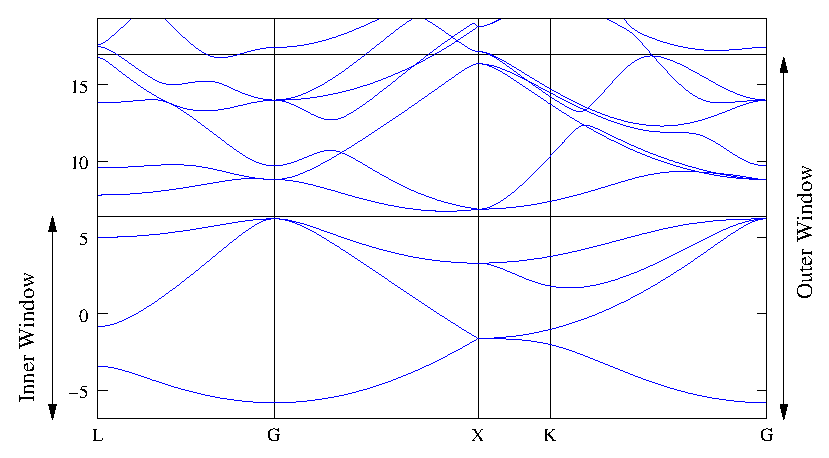
\includegraphics{si}
%\caption{Band Structure of Silicon showing the position of the outer
%and inner energy windows.}
%\label{fig:si.bnd}
%\end{center}
%\end{figure}

%\cleardoublepage


\sectiontitle{17: Iron -- Spin-orbit-coupled bands and
Fermi-surface contours}

Note: It is recommended that you go through Example 8 first (bcc Fe
without spin-orbit).

Note: This example requires a recent version of the {\tt pw2wannier90} interface.

\begin{itemize}
\item{Outline: \it{Plot the spin-orbit-coupled bands of ferromagnetic
      bcc Fe.  Plot the Fermi-surface contours on a plane in the
      Brillouin zone.}}
\item{Directory: {\tt examples/example17/}}
\item{Input files}
\begin{itemize}
\item{ {\tt Fe.scf} {\it The \pwscf\ input file for ground state
    calculation}}
\item{ {\tt Fe.nscf}  {\it The \pwscf\ input file to obtain Bloch
    states on a uniform grid}} 
\item{ {\tt Fe.pw2wan}  {\it The input file for {\tt pw2wannier90}}}

\item{ {\tt Fe.win}  {\it The {\tt wannier90} and {\tt postw90} input file}}
\end{itemize}
\end{itemize}

Note that {\tt num\_wann =18} in {\tt Fe.win}, but only nine trial
orbitals are provided. The line
  {\tt
\begin{quote}
spinors = true
\end{quote}
}tells {\tt wannier90} to use in step~3 below the specified trial
orbitals on both the up- and down-spin channels, effectively doubling
their number.

\begin{enumerate}
\item Run \pwscf\ to obtain the ferromagnetic ground state of
  iron\footnote{Please note the following counterintuitive feature in
    {\tt pwscf}: in order to obtain a ground state with magnetization
    along the {\it positive} $z$-axis, one should use a {\it negative}
    value for the variable {\tt starting\_magnetization}.}\\
  {\tt pw.x < Fe.scf > scf.out}

\item Run \pwscf\ to obtain the Bloch states on a uniform k-point
  grid\\ 
{\tt pw.x < Fe.nscf > nscf.out}

\item Run \wannier\ to generate a list of the required overlaps (written
  into the {\tt Fe.nnkp} file)\\
{\tt wannier90.x -pp Fe}

\item Run {\tt pw2wannier90} to compute:
  \begin{itemize}

  \item[{\bf --}] The overlaps $\langle u_{n{\bf k}}\vert u_{m{\bf
        k}+{\bf b}}\rangle$ between {\it spinor} Bloch states (written
    in the {\tt Fe.mmn} file)

  \item[{\bf --}] The projections for the starting guess (written in
    the {\tt Fe.amn} file)

  \item[{\bf --}] The spin matrix elements $\langle \psi_{n{\bf
        k}}\vert \sigma_i\vert \psi_{m{\bf k}}\rangle$, $i=x,y,z$
    (written in the {\tt Fe.spn} file)
%\item{The matrix elements  $\langle u_{n{\bf k}+{\bf b}_1}\vert H_{\bf k}\vert
%u_{m{\bf k}+{\bf
%          b}_2}\rangle$ (written in the {\tt
%        Fe.uHu} file)}
  \end{itemize}
{\tt pw2wannier90.x < Fe.pw2wan > pw2wan.out}

\item Run \wannier\ to compute the MLWFs.\\
{\tt wannier90.x Fe}

\item Run \postw\ to compute the energy eigenvalues and spin
  expectation values.\\
  {\tt postw90.x Fe} (serial execution) \\
  {\tt mpirun -np 8 postw90.x Fe} (example of parallel execution with
  8 MPI processes) 

\end{enumerate}

 In this example we use the module {\tt kpath} to plot the energy
  bands coloured by the expectation value of the spin along [001]:
  {\tt
\begin{quote}
kpath = true

kpath\_task = bands

kpath\_bands\_colour = spin     

kpath\_num\_points=500
\end{quote} }


To plot the bands using {\tt gnuplot} (version 4.2 or higher) issue
%
{\tt
\begin{quote}
myshell> gnuplot

gnuplot> load `Fe-bands.gnu'
\end{quote} }
%
or, using {\tt python},
%
{\tt
\begin{quote}
myshell> python Fe-bands.py
\end{quote} }

Next we plot the Fermi-surface contours on the (010) plane $k_y=0$,
using the {\tt kslice} module. Set {\tt kpath = false} and uncomment
the following instructions in {\tt Fe.win}, 
%
{\tt
\begin{quote}
kslice = true

kslice\_task = fermi\_lines

fermi\_energy = [insert your value here] 

kslice\_corner = 0.0  0.0  0.0

kslice\_b1 =     0.5 -0.5 -0.5

kslice\_b2 =     0.5  0.5  0.5

kslice\_2dkmesh = 200 200
\end{quote} }

taking the Fermi level value from {\tt scf.out}. The energy
eigenvalues are computed on a $200\times 200$ $k$-point grid covering
the BZ slice. The lines of intersection between the Fermi surface and
the (010) plane can be visualized with the {\tt gnuplot} or {\tt
  python} scripts generated at runtime,
%
{\tt
\begin{quote}
myshell> gnuplot

gnuplot> load `Fe-kslice-fermi\_lines.gnu'
\end{quote} }
%
%(do not be concerned by the warning messages, they are caused by the
%fact that not all bands cross the Fermi energy) 
or 
%
{\tt
\begin{quote}
myshell> python Fe-kslice-fermi\_lines.py
\end{quote} }
%
The Fermi lines can be colour-coded by the spin expectation value
$\langle S_z\rangle$ of the states on the Fermi surface. Add to {\tt
  Fe.win} the line {\tt
\begin{quote}
kslice\_fermi\_lines\_colour = spin
\end{quote} }
%
and re-run {\tt postw90}. The names of the {\tt gnuplot} and {\tt
  python} scripts generated at runtime are unchanged. (However, the
plotting algorithm is different in this case, and the lines are not as
smooth as before. You may want to increase {\tt kslice\_2dkmesh}.)


\subsection*{Further ideas}

\begin{itemize}

\item Redraw the Fermi surface contours on the (010) plane starting
  from a calculation without spin-orbit coupling, by adding to the
  input files {\tt iron\_\{up,down\}.win} in Example~8 the lines {\tt
\begin{quote}
kslice = true

kslice\_task = fermi\_lines

fermi\_energy = [insert your value here] 

kslice\_corner = 0.0  0.0  0.0

kslice\_b1 =     0.5 -0.5 -0.5

kslice\_b2 =     0.5  0.5  0.5

kslice\_2dkmesh = 200 200
\end{quote} }
%
before running {\tt postw90},
%
{\tt
\begin{quote}
postw90.x iron\_up

postw90.x iron\_dn
\end{quote}
}
%
The {\tt python} scripts generated at runtime draw the up- and
down-spin Fermi lines on separate figures. To draw them together, use
the script {\tt iron\_updn-kslice-fermi\_lines.py} provided with
Example~17 (or merge the two generated scripts). Compare the Fermi
lines with and without spin-orbit, and note the spin-orbit-induced
avoided crossings.

\item In Example~8 we obtained MLWFs separately for the up- and down-spin
channels of bcc Fe without spin-orbit. The Wannier-interpolated DOS
was therefore automatically separated into minority and majority
contributions.  For a spinor calculation we can still spin-decompose
the DOS, using
%
{\tt
\begin{quote}
dos = true

spin\_decomp = true

dos\_kmesh = 25 25 25
\end{quote} }
%
The data file {\tt Fe-dos.dat} created by {\tt postw90} contains the
up-spin and down-spin contributions in the third and fourth columns,
%
{\tt
\begin{quote}
myshell> gnuplot

gnuplot> plot 'Fe-dos.dat' u (-\$3):(\$1-12.6285) w l,'Fe-dos.dat' u (\$4):(\$1-12.6285) w l
\end{quote} }
%
(You should replace 12.6285 with your value of the Fermi energy).  An
alternative approach is to project the DOS onto the up-spin and
down-spin WFs separately. To find the DOS projected onto the up-spin
(odd-numbered) WFs replace {\tt spin\_decomp = true} with
%
{\tt
\begin{quote}
  dos\_project = 1,3,5,7,9,11,13,15,17
\end{quote} }
%
and re-run {\tt postw90}. This approach has the advantage that it does
not require the {\tt Fe.spn} file.


\end{itemize}

%\cleardoublepage

\sectiontitle{18: Iron -- Berry curvature, anomalous Hall
  conductivity and optical conductivity}

Note: This example requires a recent version of the {\tt pw2wannier90} interface.

\begin{itemize}
\item{Outline: \it{Calculate the Berry curvature, anomalous Hall
      conductivity, and (magneto)optical conductivity of ferromagnetic
      bcc Fe with spin-orbit coupling. In preparation for this example
      it may be useful to read Ref.~\cite{yao-prl04} and Ch.~11 of the
      User Guide.}}
\item{Directory: {\tt examples/example18/}}
\item{Input files}
\begin{itemize}
\item{ {\tt Fe.scf} {\it The \pwscf\ input file for ground state
    calculation}}
\item{ {\tt Fe.nscf}  {\it The \pwscf\ input file to obtain Bloch
    states on a uniform grid}} 
\item{ {\tt Fe.pw2wan}  {\it The input file for {\tt pw2wannier90}}}
\item{ {\tt Fe.win}  {\it The {\tt wannier90} and {\tt postw90} input file}}
\end{itemize}
\end{itemize}

The sequence of steps below is the same of Example~17.  If you have
already run that example, you can reuse the output files from steps
1--5, and only step 6 must be carried out again using the new input
file {\tt Fe.win}.

\begin{enumerate}
\item Run \pwscf\ to obtain the ground state of iron\\
{\tt pw.x < Fe.scf > scf.out}

\item Run \pwscf\ to obtain the Bloch states on a uniform k-point
  grid\\ 
{\tt pw.x < Fe.nscf > nscf.out}

\item Run \wannier\ to generate a list of the required overlaps (written
  into the {\tt Fe.nnkp} file)\\
{\tt wannier90.x -pp Fe}

\item Run {\tt pw2wannier90} to compute the overlaps between Bloch
  states and the projections for the starting guess (written in the
  {\tt Si.mmn} and {\tt  Si.amn} files)\\
{\tt pw2wannier90.x < Fe.pw2wan > pw2wan.out}

\item Run \wannier\ to compute the MLWFs\\
{\tt wannier90.x Fe}

\item Run \postw\ \\
  {\tt postw90.x Fe} (serial execution)\\
  {\tt mpirun -np 8 postw90.x Fe} (example of parallel execution with
  8 MPI processes) 

\end{enumerate}

\subsection*{Berry curvature plots}

The Berry curvature $\Omega_{\alpha\beta}({\bf k})$ of the occupied
states is defined in Eq.~(11.18) of the User Guide.  The following
lines in {\tt Fe.win} are used to calculate the energy bands and the
Berry curvature (in bohr$^2$) along high-symmetry lines in $k$-space.
{\tt
\begin{quote}
fermi\_energy = [insert your value here] 

berry\_curv\_unit = bohr2

kpath = true

kpath\_task = bands+curv

kpath\_bands\_colour = spin

kpath\_num\_points = 1000
\end{quote} }

%The path specification in {\tt Fe.win} is the same as in Example~17, and 
 

After executing {\tt postw90}, plot the Berry curvature component
$\Omega_z({\bf k})=\Omega_{xy}({\bf k})$ along the magnetization
direction using the script generated at runtime, 
%
{\tt
\begin{quote}
myshell> python Fe-bands+curv\_z.py
\end{quote} }

and compare with Fig.~2 of Ref.~\cite{yao-prl04}.  

In Example~17 we plotted the Fermi lines on the (010) plane $k_y=0$.
To combine them with a heatmap plot of (minus) the Berry curvature set
{\tt kpath = false}, uncomment the following lines in {\tt Fe.win},
\smallskip {\tt
\begin{quote}
kslice = true

kslice\_task = curv+fermi\_lines

kslice\_corner = 0.0  0.0  0.0

kslice\_b1 =     0.5 -0.5 -0.5

kslice\_b2 =     0.5  0.5  0.5

kslice\_2dkmesh = 200 200
\end{quote} }
%
re-run {\tt postw90}, and issue
%
{\tt
\begin{quote}
myshell> python Fe-kslice-curv\_z+fermi\_lines.py
\end{quote} }
\medskip
%
Compare with Fig.~3 in Ref.~\cite{yao-prl04}. Note how the Berry
curvature ``hot-spots'' tend to occur near spin-orbit-induced avoided
crossings (the Fermi lines with and without spin-orbit were generated
in Example~17).

\subsection*{Anomalous Hall conductivity}

The intrinsic anomalous Hall conductivity (AHC) is proportional to the
BZ integral of the Berry curvature. In bcc Fe with the magnetization
along $\hat{\bf z}$, the only nonzero components are
$\sigma_{xy}=-\sigma_{yx}$.  To evaluate the AHC using a $25\times
25\times 25$ $k$-point mesh, set {\tt kslice = false}, uncomment the
following lines in {\tt Fe.win}, {\tt
\begin{quote}
berry = true

berry\_task = ahc                

berry\_kmesh = 25 25 25

\end{quote} } and re-run {\tt postw90}.  The AHC is written in the
output file {\tt Fe.wpout} in vector form.  For bcc Fe with the
magnetization along [001], only the $z$-component $\sigma_{xy}$ is
nonzero.

As a result of the strong and rapid variations of the Berry curvature
across the BZ, the AHC converges rather slowly with $k$-point
sampling, and a $25\times 25\times 25$ does not yield a well-converged
value.

  \begin{itemize}

  \item[{\bf --}] Increase the BZ mesh density by changing {\tt
      berry\_kmesh}.

  \item[{\bf --}] To accelerate the convergence, adaptively refine the
    mesh around spikes in the Berry curvature, by adding to {\tt
      Fe.win} the lines \smallskip {\tt
      \begin{quote}
        berry\_curv\_adpt\_kmesh = 5  
        
        berry\_curv\_adpt\_kmesh\_thresh = 100.0
      \end{quote} }

  \end{itemize}
    
    This adds a $5\times 5\times 5$ fine mesh around those points
    where $\vert{\bm \Omega}({\bf k})\vert$ exceeds 100~bohr$^2$. The
    percentage of points triggering adaptive refinement is reported in
    {\tt Fe.wpout}.

    Compare the converged AHC value with those obtained in
    Refs.~\cite{wang-prb06} and~\cite{yao-prl04}.

    The Wannier-interpolation formula for the Berry curvature
    comprises three terms, denoted $D$-$D$, $D$-$\overline{A}$, and
    $\overline{\Omega}$ in Ref.~\cite{wang-prb06}, and $J2$, $J1$, and
    $J0$ in Ref.~\cite{lopez-prb12}.  To report in {\tt Fe.wpout} the
    decomposition of the total AHC into these three terms, set {\tt
      iprint} (verbosity level) to a value larger than one in {\tt
      Fe.win}.

\subsection*{Optical conductivity}

The optical conductivity tensor of bcc Fe with magnetization along
$\hat{\bf z}$ has the form
%
$$
\bm{\sigma}=\bm{\sigma}^{\rm S}+\bm{\sigma}^{\rm A}=
\left(
\begin{array}{ccc}
\sigma_{xx} & 0 & 0\\
0 & \sigma_{xx} & 0\\
0 & 0 & \sigma_{zz}
\end{array}
\right)+
\left(
\begin{array}{ccc}
0 & \sigma_{xy} & 0 \\
-\sigma_{xy} & 0 & 0\\
0 & 0 & 0
\end{array}
\right)$$
%
where ``S'' and ``A'' stand for the symmetric and antisymmetric parts
and $\sigma_{xx}=\sigma_{yy}\not=\sigma_{zz}$. The dc AHC calculated
earlier corresponds to $\sigma_{xy}$ in the limit $\omega\rightarrow
0$. At finite frequency $\sigma_{xy}=-\sigma_{yx}$ acquires an
imaginary part which describes magnetic circular dichoism (MCD).

To compute the complex optical conductivity for $\hbar\omega$
up to 7~eV, replace 
{\tt
\begin{quote}
berry\_task = ahc
\end{quote} }
%
with
%
{\tt
\begin{quote}
berry\_task = kubo
\end{quote} }
%
add the line
%
{\tt
\begin{quote}
kubo\_freq\_max = 7.0
\end{quote} }
%
and re-run {\tt postw90}. Reasonably converged spectra can be
obtained with a $125\times 125\times 125$ $k$-point mesh. Let us first
plot the ac AHC in S/cm, as in the lower panel of Fig.~5 in
Ref.~\cite{yao-prl04}, {\tt
\begin{quote}
myshell> gnuplot

gnuplot> plot `Fe-kubo\_A\_xy.dat' u 1:2 w l
\end{quote} }

Comapare the $\omega\rightarrow 0$ limit with the result obtained
earlier by integrating the Berry curvature.\footnote{The calculation
  of the AHC using {\tt berry\_task = kubo} involves a truncation of
  the sum over empty states in the Kubo-Greenwood formula: see
  description of the keyword {\tt kubo\_eigval\_max} in the User
  Guide. As discussed around Eq.~(11.17) of the User Guide, no
  truncation is done with {\tt berry\_task = ahc}.}


Next we plot the MCD spectrum. Following Ref.~\cite{yao-prl04}, we
plot ${\rm Im}[\omega\sigma_{xy}(\hbar\omega)]$, in units of
$10^{29}$~sec$^{-2}$. The needed conversion factor is $9\times
10^{-18}\times e/\hbar\simeq 0.0137$ ($e$ and $\hbar$ in SI units),
{\tt
\begin{quote}
gnuplot> set yrange[-5:15]

gnuplot> plot `Fe-kubo\_A\_xy.dat' u 1:(\$1)*(\$3)*0.0137 w l
\end{quote} }

\subsection*{Further ideas}

\begin{itemize}

\item Recompute the AHC and optical spectra of bcc Fe using projected
  $s$, $p$, and $d$-type Wannier functions instead of the hybridrized
  MLWFs (see Example~8), and compare the results.

\item A crude way to model the influence of heterovalent alloying on
  the AHC is to assume that its only effect is to donate or deplete
  electrons, i.e., to shift the Fermi level of the pure
  crystal~\cite{yao-prb07}.

Recalculate the AHC of bcc Fe for a range of Fermi energies within
$\pm 0.5$~eV of the true Fermi level. This calculation can be
streamlined by replacing in {\tt Fe.win} {\tt
\begin{quote}
fermi\_energy = [insert your value here]
\end{quote} }
%
with
%
{\tt
\begin{quote}
fermi\_energy\_min = [insert here your value minus 0.5]

fermi\_energy\_max = [insert here your value plus 0.5]
\end{quote} }
%
Use a sufficiently dense BZ mesh with adaptive refinement. To plot
$\sigma_{xy}$ versus $\varepsilon_F$, issue
%
{\tt
\begin{quote}
myshell> gnuplot

gnuplot> plot `Fe-ahc-fermiscan.dat' u 1:4 w lp
\end{quote} }

\end{itemize}


%\cleardoublepage

\sectiontitle{19: Iron -- Orbital magnetization}

Note: This example requires a recent version of the {\tt pw2wannier90} interface.

\begin{itemize}
\item{Outline: \it{Calculate the orbital magnetization of
      ferromagnetic bcc Fe by Wannier interpolation.}}
\item{Directory: {\tt examples/example19/}}
\item{Input files}
\begin{itemize}
\item{ {\tt Fe.scf} {\it The \pwscf\ input file for ground state
    calculation}}
\item{ {\tt Fe.nscf}  {\it The \pwscf\ input file to obtain Bloch
    states on a uniform grid}} 
\item{ {\tt Fe.pw2wan}  {\it The input file for {\tt pw2wannier90}}}
\item{ {\tt Fe.win} {\it The {\tt wannier90} and {\tt postw90} input
      file}}
\end{itemize}
\end{itemize}

The sequence of steps below is the same of Examples~17 and 18.  If you
have already run one of those examples, you can reuse the output files
from steps 1--3 and 5. Steps~4 and 6 should be carried out again using
the new input files {\tt Fe.pw2wan} and {\tt Fe.win}.

\begin{enumerate}
\item Run \pwscf\ to obtain the ground state of iron\\
{\tt pw.x < Fe.scf > scf.out}

\item Run \pwscf\ to obtain the Bloch states on a uniform k-point
  grid\\ 
{\tt pw.x < Fe.nscf > nscf.out}

\item Run \wannier\ to generate a list of the required overlaps (written
  into the {\tt Fe.nnkp} file).\\
{\tt wannier90.x -pp Fe}


\item Run {\tt pw2wannier90} to compute:
  \begin{itemize}

  \item[{\bf --}] The overlaps $\langle u_{n{\bf k}}\vert u_{m{\bf k}+{\bf
          b}}\rangle$ (written in the {\tt Fe.mmn} file)

  \item[{\bf --}] The projections for the starting guess (written in the {\tt
        Fe.amn} file)

  \item[{\bf --}] The matrix elements $\langle u_{n{\bf k}+{\bf b}_1}\vert
      H_{\bf k}\vert u_{m{\bf k}+{\bf b}_2}\rangle$ (written in the
      {\tt Fe.uHu} file)

%  \item[{\bf --}] The spin matrix elements $\langle \psi_{n{\bf
%        k}}\vert \sigma_i\vert \psi_{m{\bf k}}\rangle$ (written in the
%    {\tt Fe.spn} file)

  \end{itemize}
{\tt pw2wannier90.x < Fe.pw2wan > pw2wan.out}

\item Run \wannier\ to compute the MLWFs.\\
{\tt wannier90.x Fe}

\item Run \postw\ to compute the orbital magnetization.\\
  {\tt postw90.x Fe} (serial execution)\\
  {\tt mpirun -np 8 postw90.x Fe} (example of parallel execution with
  8 MPI processes) 


\end{enumerate}

The orbital magnetization is computed as the BZ integral of the
quantity ${\bf M}^{\rm orb}({\bf k})$ defined in Eq.~(11.20) of the
User Guide. The relevant lines in {\tt Fe.win} are
%
{\tt
\begin{quote}
berry = true

berry\_task = morb

berry\_kmesh = 25 25 25

fermi\_energy = [insert your value here]
\end{quote} }
%
After running {\tt postw90}, compare the value of the orbital
magnetization reported in {\tt Fe.wpout} with the spin magnetization
in {\tt scf.out}. Set {\tt iprint = 2} to report the decomposition of
${\bf M}^{\rm orb}$ into the terms $J0$, $J1$, and $J2$ defined in
Ref.~\cite{lopez-prb12}.
%\footnote{Alternatively, the
%spin magnetization can be computed by {\tt postw90}. This requires adding the
%instruction {\tt spin\_moment = T} to {\tt Fe.win}, assuming that {\tt pw2wannier90}
%was executed with {\tt write\_spn = .true.} in {\tt Fe.pw2wan}.} 
%Both point along $\hat{\bf
%  z}$, but the orbital contribution is much smaller (it is strongly
%quenched by the crystal field).

To plot $M_z^{\rm orb}({\bf k})$ along high-symmetry lines set {\tt
  berry = false} and uncomment in {\tt Fe.win} the block of
instructions containing {\tt
\begin{quote}
kpath = true

kpath\_task = bands+morb
\end{quote}
}
After running {\tt postw90}, issue
%
{\tt
\begin{quote}
myshell> python Fe-bands+morb\_z.py
\end{quote} } 
%
Compare with Fig.~2 of Ref.~\cite{lopez-prb12}, bearing in mind the
factor of $-1/2$ difference in the definition of ${\bf M}^{\rm
  orb}({\bf k})$ (see Ch.~11 in the User Guide).

To plot $M_z^{\rm orb}({\bf k})$ together with the Fermi contours on the
(010) BZ plane set {\tt kpath = false}, uncomment in {\tt
  Fe.win} the block of instructions containing 
{\tt
\begin{quote}
kslice = true

kslice\_task = morb+fermi\_lines
\end{quote}
} 
re-run {\tt postw90}, and issue
{\tt
\begin{quote}
myshell> python Fe-kslice-morb\_z+fermi\_lines.py
\end{quote} }
%
$M_z^{\rm orb}({\bf k})$ is much more evenly distributed in $k$-space
than the Berry curvature (see Example 18). As a result, the integrated
orbital magnetization converges more rapidly with the BZ sampling.


%%\sectiontitle{20: Disentanglement only in small (spherical) regions of $k$ space}
%%
\sectiontitle{20: Disentanglement restricted inside spherical regions of $k$ space}
\subsection*{LaVO$_3$}
\begin{itemize}
\item{Outline: \it{Obtain disentangled MLWFs for strained LaVO$_3$.}}
\item{Directory: {\tt examples/example20/}}
\item{Input Files}
\begin{itemize}
\item{ {\tt LaVO3.scf}  {\it The \pwscf\ input file for ground state
    calculation}} 
\item{ {\tt LaVO3.nscf}  {\it The \pwscf\ input file to obtain Bloch
    states on a uniform grid}} 
\item{ {\tt LaV03.pw2wan}  {\it Input file for {\tt pw2wannier90}}}
\item{ {\tt LaVO3.win}  {\it The {\tt wannier90} input file}}
\end{itemize}

\end{itemize}

\begin{enumerate}
\item Run \pwscf\ to obtain the ground state of LaVO$_3$.\\
{\tt pw.x < LaVO3.scf > scf.out}

\item Run \pwscf\ to obtain the Bloch states on a uniform k-point
  grid.\\ 
{\tt pw.x < LaVO3.nscf > nscf.out}

\item Run \wannier\ to generate a list of the required overlaps (written
  into the {\tt LaVO3.nnkp} file).\\
{\tt wannier90.x -pp LaVO3}

\item Run {\tt pw2wannier90} to compute the overlap between Bloch
  states and the projections for the starting guess (written in the
  {\tt LaVO3.mmn} and {\tt  LaVO3.amn} files).\\
{\tt pw2wannier90.x < LaVO3.pw2wan > pw2wan.out}

\item Run \wannier\ to compute the MLWFs.\\
{\tt wannier90.x LaVO3}

\end{enumerate}

Inspect the output file {\tt LaVO3.wout}. In the initial summary, you
will see that the disentanglement was performed only within one sphere
of radius 0.2 arount the point $A=(0.5, 0.5, 0.5)$ in reciprocal space:
\begin{verbatim}
 |  Number of spheres in k-space              :                 1             |
 |   center n.   1 :     0.500   0.500   0.500,    radius   =   0.200         |
\end{verbatim}

Compare the band structure that Wannier90 produced with the one
obtained using Quantum ESPRESSO. You should get something similar to Fig.~\ref{fig:lavo3}.
%%
Notice how the $t_{2g}$-bands are entangled with other bands at $A$ and the Wannier-interpolated band structure deviates from the Bloch bands only in a small region around that $k$-point.
It is important to keep in mind that all symmetry equivalent $k$-points within the first Brillouin zone must be written explicitly in the list of sphere centers. 
For instance, the $A$ point in the simple tetragonal lattice of this example is non-degenerate, while the $X$ point has degeneracy two, hence one must specify both $(1/2,0,0)$ and $(0,1/2,0)$ (see the SrMnO$_3$ example here below).

\begin{figure}[h]
\begin{center}
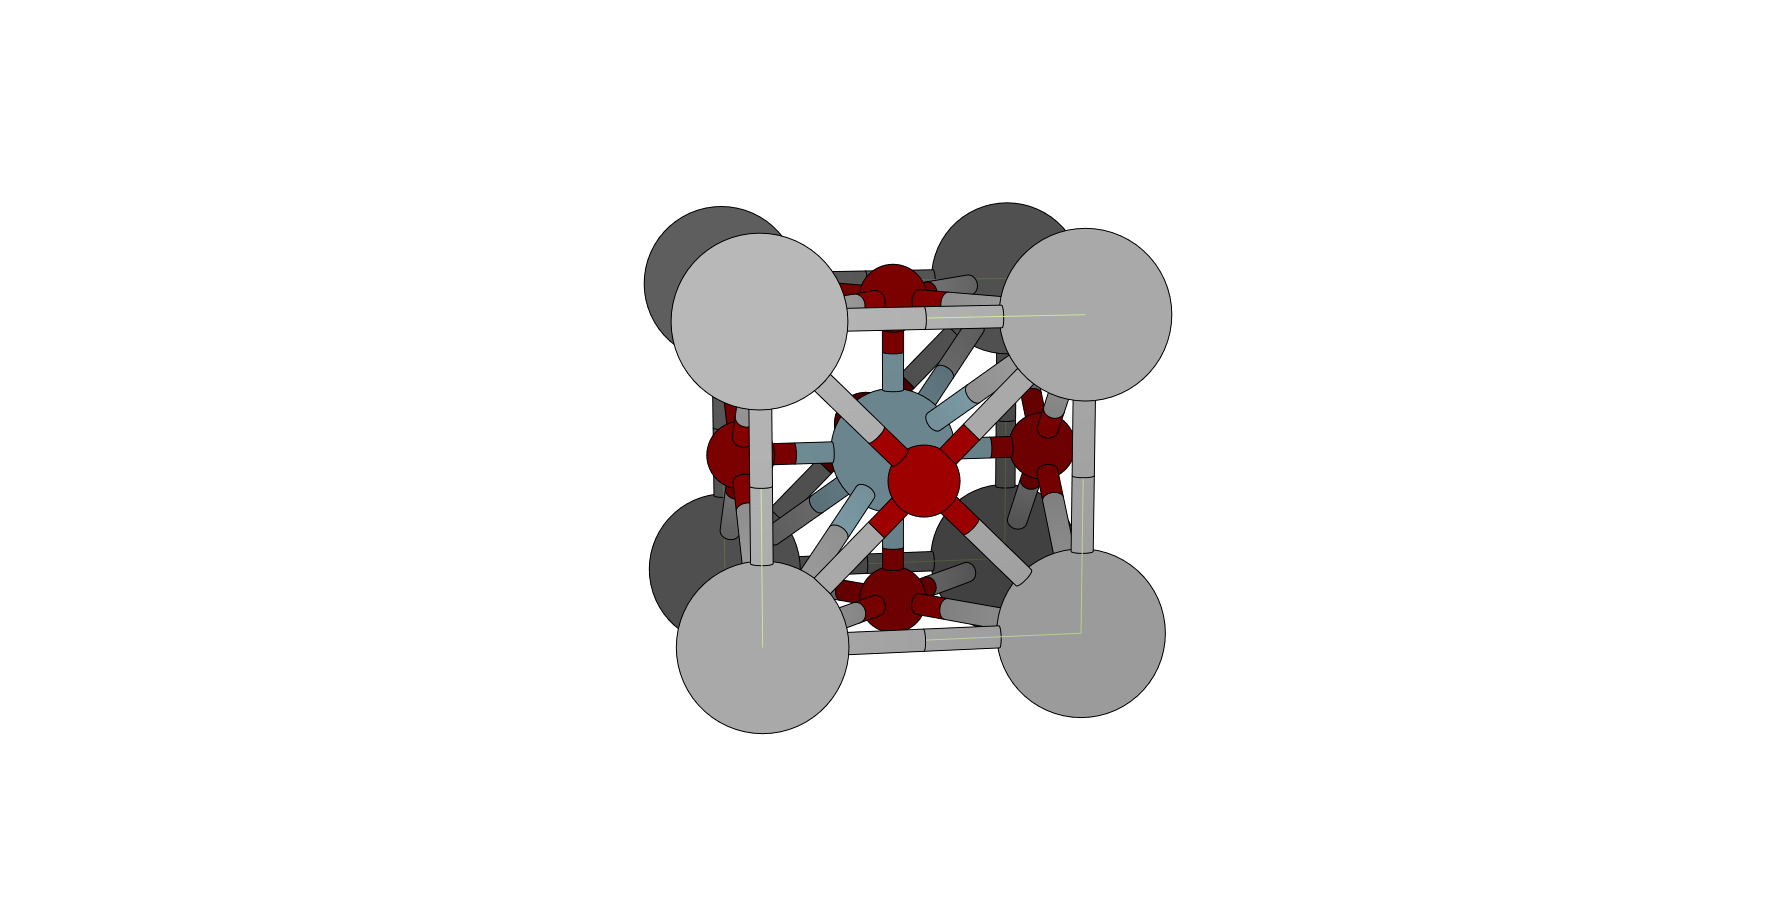
\includegraphics[width=10cm]{LaVO3}
\caption{Band structure of epitaxially-strained (tetragonal) LaVO$_3$. Black: Bloch bands; red circles: Wannier-interpolated band structure. The disentanglement was performed only for $k$-points within a sphere of radius 0.2 \AA$^{-1}$ centered in $A$.} 
\label{fig:lavo3}
\end{center}
\end{figure}

\subsection*{Further ideas}

\begin{itemize}
%\item Try to disentangle the Wannier functions without disentanglement, and with standard disentanglement without using the spheres. You will notice that without disentanglement Wannier functions will not converge. With standard disentanglement (without spheres), also bands away from the A point in $k-$space are perturbed, even in regions of $k-$space where there is no entanglement. 
\item Try to obtain the Wannier functions using the standard disentanglement procedure (without spheres, \verb+dis_spheres_num = 0+). You will notice that the Wannier-interpolated band structure now shows deviations also in regions of $k$-space far away from $A$, where disentanglement is actually not necessary. If you disable the disentanglement completely, instead, the Wannierisation procedure does not converge.

\item In order to illustrate all possible cases, it is instructive to apply this method to SrMnO$_3$, where the $t_{2g}$ bands are entangled with the above-lying $e_g$ bands, and also with the deeper O-$2p$ states.
  In the SrMnO$_3$ subfolder, you can find input files for building three different sets of Wannier functions: only $t_{2g}$ states, only $e_g$ states, or all V-$3d$-derived states ($t_{2g} + e_g$). In each case one needs to specify different disentanglement spheres, according to which region(s) in $k$-space show entanglement of the targeted bands. 
  Also the index \verb+dis_sphere_first_wan+ needs to be adapted to the new disentanglement window, which here contains also states below the lowest-lying Wannier function (at variance with the LaVO$_3$ case).
\end{itemize}

%\cleardoublepage

\sectiontitle{21: Gallium Arsenide -- Symmetry-adapted Wannier functions}

Note: This example requires a recent version of the {\tt pw2wannier90} interface.

\begin{itemize}
\item{Outline: \it{Obtain symmetry-adapted Wannier functions out of four valence bands of GaAs. 
For the theoretical background of the symmetry-adapted Wannier functions, see R. Sakuma,  Phys. Rev. B {\bf 87}, 235109 (2013).}}
\item{Directory: {\tt examples/example21/atom\_centered\_As\_sp/} \\
\phantom{Directory: }{\tt examples/example21/atom\_centered\_Ga\_p/}    \\
\phantom{Directory: }{\tt examples/example21/atom\_centered\_Ga\_s/}    \\
\phantom{Directory: }{\tt examples/example21/atom\_centered\_Ga\_sp/}    \\
\phantom{Directory: }{\tt examples/example21/bond\_centered/}    
}
\item{Input Files}
\begin{itemize}
\item{ {\tt GaAs.scf}  {\it The \pwscf\ input file for ground state
    calculation}} 
\item{ {\tt GaAs.nscf}  {\it The \pwscf\ input file to obtain Bloch
    states on a uniform grid}} 
\item{ {\tt GaAs.pw2wan}  {\it The input file for {\tt pw2wannier90}}}
\item{ {\tt GaAs.win}  {\it The {\tt wannier90} input file}}
\end{itemize}
\end{itemize}

\begin{enumerate}
\item Run \pwscf\ to obtain the ground state of GaAs\\
{\tt pw.x < GaAs.scf > scf.out}

\item Run \pwscf\ to obtain the Bloch states on a uniform k-point grid\\
{\tt pw.x < GaAs.nscf > nscf.out}

\item Run \wannier\ to generate a list of the required overlaps (written
  into the {\tt GaAs.nnkp} file).\\ 
{\tt wannier90.x -pp GaAs}

\item Run {\tt pw2wannier90} to compute the overlap between Bloch
  states, the projections for the starting guess, and the symmetry information needed for symmetry-adapted mode (written in the
  {\tt GaAs.mmn}, {\tt GaAs.amn}, and {\tt GaAs.dmn} files, respectively).\\  
{\tt pw2wannier90.x < GaAs.pw2wan > pw2wan.out}

\item Run \wannier\ to compute the MLWFs.\\
{\tt wannier90.x GaAs}
\end{enumerate}

Each directory creates different kind of symmetry-adapted Wannier function. 
See more detail in {\tt examples/example21/README}. 
%Compare the results with those of Sec. III.A in R. Sakuma, Phys. Rev. B {\bf 87}, 235109 (2013). 


%\cleardoublepage

\sectiontitle{22: Copper -- Symmetry-adapted Wannier functions}

Note: This example requires a recent version of the {\tt pw2wannier90} interface.

\begin{itemize}
\item{Outline: \it{Obtain symmetry-adapted Wannier functions for Cu. By symmetry-adapted mode, for example, we can make atomic centered $s$-like Wannier function, which is not possible in the usual procedure to create maximally localized Wannier functions.
For the theoretical background of the symmetry-adapted Wannier functions, see R. Sakuma,  Phys. Rev. B {\bf 87}, 235109 (2013).}}
\item{Directory: {\tt examples/example22/s\_at\_0.00/} \\
\phantom{Directory: }{\tt examples/example22/s\_at\_0.25/}    \\
\phantom{Directory: }{\tt examples/example22/s\_at\_0.50/}    
}
\item{Input Files}
\begin{itemize}
\item{ {\tt Cu.scf}  {\it The \pwscf\ input file for ground state
    calculation}} 
\item{ {\tt Cu.nscf}  {\it The \pwscf\ input file to obtain Bloch
    states on a uniform grid}} 
\item{ {\tt Cu.pw2wan}  {\it The input file for {\tt pw2wannier90}}}
\item{ {\tt Cu.sym}  {\it Used only in {\tt examples/example22/s\_at\_0.25/}. {\tt pw2wannier90} reads this file when {\tt ``read\_sym = .true.''} in {\tt Cu.pw2wan}. By default, {\tt ``read\_sym = .false.'' and {\tt Cu.sym} is the output of {\tt pw2wannier90}}, in which the symmetry operations employed in the calculation are written for reference. } } 
\item{ {\tt Cu.win}  {\it The {\tt wannier90} input file}}
\end{itemize}
\end{itemize}

\begin{enumerate}
\item Run \pwscf\ to obtain the ground state of Cu\\
{\tt pw.x < Cu.scf > scf.out}

\item Run \pwscf\ to obtain the Bloch states on a uniform k-point grid\\
{\tt pw.x < Cu.nscf > nscf.out}

\item Run \wannier\ to generate a list of the required overlaps (written
  into the {\tt Cu.nnkp} file).\\ 
{\tt wannier90.x -pp Cu}

\item Run {\tt pw2wannier90} to compute the overlap between Bloch
  states, the projections for the starting guess, and the symmetry information needed for symmetry-adapted mode (written in the
  {\tt Cu.mmn}, {\tt Cu.amn}, and {\tt Cu.dmn} files, respectively).\\  
{\tt pw2wannier90.x < Cu.pw2wan > pw2wan.out}

\item Run \wannier\ to compute the MLWFs.\\
{\tt wannier90.x Cu}
\end{enumerate}

Each directory creates $s$-like symmetry-adapted Wannier function centered at different position on top of atomic centered $d$-like Wannier functions. 
See more detail in {\tt examples/example22/README}. 
%Compare the results with those of Sec. III.B in R. Sakuma,  Phys. Rev. B {\bf 87}, 235109 (2013). 


\sectiontitle{23: Silicon -- $G_0W_0$ bands structure interpolation}

Note: This example requires a recent version of the {\tt ypp} post-processing code of {\tt yambo}.

\begin{itemize}
\item{Outline: \it{Interpolate the bands structure of silicon obtained from many-body perturbation theory at the $G_0W_0$ level. Using the {\tt yambo} code, the quasi-particle corrections (QP) are summed to Kohn-Sham eigenvalues, while the wavefunctions remain the same. }}
\item{Directory: {\tt examples/example23/}}
\item{Input Files}
\begin{itemize}
\item{ {\tt silicon.scf}  {\it The \pwscf\ input file for the ground state
    calculation}} 
\item{ {\tt silicon.nscf }  {\it The \pwscf\ input file to obtain Bloch
    states on a uniform grid}}
\item{ {\tt silicon.gw.nscf }  {\it The \pwscf\ input file to obtain Bloch
    states on a reduced grid with many empty bands}}  
\item{ {\tt silicon.pw2wan}  {\it The input file for {\tt pw2wannier90}}}
\item{ {\tt silicon.win}  {\it The {\tt wannier90} input file}}
\item{ {\tt silicon.gw.win}  {\it The {\tt wannier90} input file} (for the $G_0W_0$ step)}
\item{ {\tt yambo.in}  {\it The {\tt yambo} input file}}
\item{ {\tt ypp.in}  {\it The {\tt ypp} input file}}
\end{itemize}
\end{itemize}

\begin{enumerate}
\item Copy the input files from the {\tt INPUT directory} into a working directory (e.g. {\tt WORK})
\item Run \pwscf\ to obtain the ground state charge of silicon \\
{\tt pw.x < silicon.scf > scf.out}
\item Run \pwscf\ to obtain the Bloch states reduced grid. We use a 8x8x8 with many bands (many empty bands are needed to perform a $G_0W_0$ with {\tt yambo})\\
{\tt pw.x < silicon.gw.nscf > nscf.gw.out}
\item Use the {\tt k\_mapper.py} utility to find the indexes of a 4x4x4 uniform grid into the 8x8x8 reduced grid \\
{\tt ./k\_mapper.py 4 4 4 "../examples/example23/WORK/nscf.gw.out"}\\
Use the output to complete the {\tt yambo.in} input file (you also need to specify the on how many bands you want to compute the QP corrections, here you can use all the bands from 1 to 14). Then, you should have obtained something like:\\
 {\tt 
1| 1|  1|14| \\
3| 3|  1|14| \\ 
5| 5|  1|14| \\ 
13| 13|  1|14| \\
...\tt}
\item Enter the {\tt si.save} directory and run {\tt p2y}. A {\tt SAVE} folder is created, you can move it up in the {\tt /WORK/} directory.\\
\item Run a $G_0W_0$ calculation from the {\tt /WORK/} directory (remember, we are using a 8x8x8 grid but computing QP corrections only on a 4x4x4 grid)\\
{\tt yambo }


\item Run \pwscf\ to obtain the Bloch states on a uniform k-point grid\\
{\tt pw.x < silicon.nscf > nscf.out}

\item Run \wannier\ to generate a list of the required overlaps (written
  into the {\tt silicon.nnkp} file).\\ 
{\tt wannier90.x -pp silicon}

\item Run {\tt pw2wannier90} to compute the overlap between Bloch
  states, the projections for the starting guess (written in the
  {\tt silicon.mmn} and {\tt silicon.amn} respectively).\\  
{\tt pw2wannier90.x < silicon.pw2wan > pw2wan.out}

\item Run \wannier\ to compute the MLWFs.\\
{\tt wannier90.x silicon}\\
At this point, you should have obtained the interpolated valence bands for silicon at the DFT level.
\item Run a {\tt ypp} calculation (just type {\tt ypp})\\
You should obtain a file {\tt silicon.gw.unsorted.eig} which contains the QP corrections on a uniform 4x4x4 grid.
\item Run the gw2wannier90.py script to reorder, align and correct all matrices and files using the QP corrections\\
{\tt ../../../utility/gw2wannier90.py silicon mmn amn}
\item Run \wannier\ to compute the MLWFs.\\
{\tt wannier90.x silicon.gw}\\
At this point, you should have obtained the interpolated valence bands for silicon at the $G_0W_0$ level.
\end{enumerate}
After you completed the tutorial for the valence bands only, you can repeat the final steps to interpolate also some conduction bands using disentanglement (the code is already present as comments in the input files).
%\cleardoublepage


\sectiontitle{24: Tellurium -- gyrotropic effects}


\begin{itemize}
\item{Outline: {\it Calculate the gyrotropic effects in trigonal right-handed Te} Similar to the calculations of \cite{tsirkin-arxiv17}}
\item{Directory: {\tt examples/example24/}}
\item{Input files}
\begin{itemize}
\item{ {\tt Te.scf} {\it The \pwscf\ input file for ground state
    calculation}}
\item{ {\tt Te.nscf}  {\it The \pwscf\ input file to obtain Bloch
    states on a uniform grid}} 
\item{ {\tt Te.pw2wan}  {\it The input file for {\tt pw2wannier90}}}
\item{ {\tt Te.win} {\it The {\tt wannier90} input
      file}}
\end{itemize}
\end{itemize}

To make things easy, the example treats Te without spin-orbit



\begin{enumerate}
\item Run \pwscf\ to obtain the ground state of tellurium\\
{\tt pw.x < Te.scf > scf.out}

\item Run \pwscf\ to obtain the Bloch states on a uniform {\tt 3x3x4} k-point
  grid\\ 
{\tt pw.x < Te.nscf > nscf.out}

\item Run \wannier\ to generate a list of the required overlaps (written
  into the {\tt Te.nnkp} file).\\
{\tt wannier90.x -pp Te}

\item Run {\tt pw2wannier90} to compute:
  \begin{itemize}

  \item[{\bf --}] The overlaps $\langle u_{n{\bf k}}\vert u_{m{\bf k}+{\bf
          b}}\rangle$ (written in the {\tt Te.mmn} file)

  \item[{\bf --}] The projections for the starting guess (written in the {\tt
        Te.amn} file)

  \item[{\bf --}] The matrix elements $\langle u_{n{\bf k}+{\bf b}_1}\vert
      H_{\bf k}\vert u_{m{\bf k}+{\bf b}_2}\rangle$ (written in the
      {\tt Te.uHu} file)

  \item[{\bf --}] The spin matrix elements $\langle \psi_{n{\bf
        k}}\vert \sigma_i\vert \psi_{m{\bf k}}\rangle$ (would be written in the
    {\tt Te.spn} file, but only if spin-orbit is included, which is not the case for the present example)

  \end{itemize}
{\tt pw2wannier90.x < Te.pw2wan > pw2wan.out}

\item Run \wannier\ to compute the MLWFs.\\
{\tt wannier90.x Te}

\item  Add the following lines to the {\tt wannier90.win} file:\\
{\tt gyrotropic=true  \\
gyrotropic\_task=-C-dos-D0-Dw-K \\
fermi\_energy\_step=0.0025\\
fermi\_energy\_min=5.8\\
fermi\_energy\_max=6.2\\
gyrotropic\_freq\_step=0.0025\\
gyrotropic\_freq\_min=0.0\\
gyrotropic\_freq\_max=0.1\\
gyrotropic\_smr\_fixed\_en\_width=0.01\\
gyrotropic\_smr\_max\_arg=5\\
gyrotropic\_degen\_thresh=0.001\\
gyrotropic\_box\_b1=0.2 0.0 0.0\\
gyrotropic\_box\_b2=0.0 0.2 0.0\\
gyrotropic\_box\_b3=0.0 0.0 0.2\\
gyrotropic\_box\_center=0.33333 0.33333 0.5\\
gyrotropic\_kmesh=50 50 50
}



\item Run \postw\ \\to compute the gyrotropic properties: tensors $D$, $\widetilde{D}$, $K$, $C$ (See the User Guide):.\\
  {\tt postw90.x Te} (serial execution)\\
  {\tt mpirun -np 8 postw90.x Te} (example of parallel execution with
  8 MPI processes) \\


The integration in the $k$-space is limited to a small area around the H point. Thus it is valid only for Fermi levels near the band gap. 
And one needs to multiply the results by 2, to account for the H' point. To integrate over the entire Brillouin zone, one needs to remove the 
{\tt gyrotropic\_box\_$\ldots$} parameters

\item Now change the above lines to \\ {\tt
gyrotropic=true\\
gyrotropic\_task=-NOA\\
fermi\_energy=5.95\\
gyrotropic\_freq\_step=0.0025\\
gyrotropic\_freq\_min=0.0\\
gyrotropic\_freq\_max=0.3\\
gyrotropic\_smr\_fixed\_en\_width=0.01\\
gyrotropic\_smr\_max\_arg=5\\
gyrotropic\_band\_list=4-9\\
gyrotropic\_kmesh=50 50 50\\
}

and compute the interband natural optical activity\\

  {\tt postw90.x Te} (serial execution)\\
  {\tt mpirun -np 8 postw90.x Te} (example of parallel execution with
  8 MPI processes) \\





\end{enumerate}

\sectiontitle{25: Gallium Arsenide -- Nonlinear shift current}

\begin{itemize}

\item Outline: \textit{Calculate the nonlinear shift current of inversion asymmetric fcc Gallium Arsenide. In preparation for this example it may be useful to read Ref.
\cite{ibanez-azpiroz_ab_2018} }



\item Directory: \verb|examples/example25/|

\item Input files:

\begin{itemize}

\item[--] \verb|GaAs.scf| \textit{The {\tt PWSCF} input file for ground state calculation}
\item[--] \verb|GaAs.nscf| \textit{The {\tt PWSCF} input file to obtain Bloch states on a uniform grid}
\item[--] \verb|GaAs.pw2wan| \textit{The input file for} \verb|pw2wannier90|
\item[--] \verb|GaAs.win| \textit{The} \verb|wannier90| \textit{and} \verb|postw90| \textit{input file}


\end{itemize}


\begin{enumerate}

\item Run {\tt PWSCF} to obtain the ground state of Gallium Arsenide

\verb|pw.x < GaAs.scf > scf.out|


\item Run {\tt PWSCF} to obtain the ground state of Gallium Arsenide

\verb|pw.x < GaAs.nscf > nscf.out|

\item Run {\tt Wannier90} to generate a list of the required overlaps (written into the \verb|GaAs.nnkp| file)

\verb|wannier90.x -pp GaAs|


\item Run {\tt pw2wannier90} to compute:

\begin{itemize}
\item[--] The overlaps $\langle u_{n\bf{k}}|u_{n\bf{k+b}}\rangle$ between spinor 
Bloch states (written in the \verb|GaAs.mmn| file) 
\item[--] The projections for the starting guess (written in the \verb|GaAs.amn| file)

\end{itemize}


\verb|pw2wannier90.x < GaAs.pw2wan > pw2wan.out|

\item Run {\tt wannier90} to  compute MLWFs

\verb|wannier90.x GaAs|

\item Run {\tt postw90} to compute nonlinear shift current

\verb|postw90.x GaAs| (serial execution)

\verb|mpirun -np 8 postw90.x GaAs| (example of parallel execution with 8 MPI processes)

\end{enumerate}




\end{itemize}


\subsection*{Shift current $\sigma^{abc}$}

The shift current tensor of GaAs has only one independent component that is finite, namely $\sigma^{xyz}$. 
For its computation, set
\begin{verbatim}
berry = true
berry_task = sc
\end{verbatim}
Like the linear optical conductivity, the shift current is a frequency-dependent quantity. 
The frequency window and step is controlled by \verb|kubo_freq_min|, \verb|kubo_freq_max| and 
\verb|kubo_freq_step|, as explained in the users guide. 

The shift current requires an integral over the Brillouin zone. The interpolated k-mesh is controlled by \verb|berry_kmesh|,
which has been set to 
\begin{verbatim}
berry_kmesh = 100 100 100
 \end{verbatim}
We also need to input the value of the Fermi level in eV:
\begin{verbatim}
fermi_energy = [insert your value here]
\end{verbatim}

Due to the sum over intermediate states involved in the calculation of the shift current, 
one needs to consider a small broadening parameter to avoid numerical problems due to possible degeneracies
(see parameter $\eta$ in Eq. (36) of Ref. \cite{ibanez-azpiroz_ab_2018} and related discussion).
This parameter is controlled by \verb|sc_eta|. It is normally found that values between 0.01 eV and 0.1 eV 
yield an stable spectrum. The default value is set to  $0.04$ eV.

Finally, \verb|sc_phase_conv| controls the phase convention used for the Bloch sums. 
\verb|sc_phase_conv=1| uses the so-called tight-binding convention, whereby the Wannier centres are included
into the phase, while   \verb|sc_phase_conv=2| leaves the Wannier centres out of the phase.
These two possible conventions are explained in Ref. \cite{pythtb}. 
Note that the overall shift-current spectrum does not depend on the chosen convention,
but the individual terms that compose it do.


On output, the program generates a set of 18 files named \verb|SEED-sc_***.dat|, 
which correspond to the different tensor components  of the shift current
(note that the 9 remaining components until totaling $3\times3\times3=27$ 
can be obtained from the 18 outputed by taking into account that $\sigma^{abc}$ is 
symmetric under $b\leftrightarrow c$ index exchange).
For plotting the only finite shift-current component of GaAs $\sigma^{xyz}$ (units of A/V$^{2}$) as in the upper 
panel of Fig. 3 in Ref. \cite{ibanez-azpiroz_ab_2018},
\begin{verbatim}
myshell> gnuplot
gnuplot> plot 'GaAs-sc_xyz.dat' u 1:2 w l
\end{verbatim} 


\sectiontitle{26: Gallium Arsenide -- Selective localization and constrained centres}

\begin{itemize}

\item Outline: \textit{Application of the selectively localised Wannier function (SLWF) method to gallium arsenide (GaAs), following the example in Ref. \cite{Marianetti}, which is essential reading for this tutorial example.}


\item Directory: \verb|examples/example26/|


\item Input files:

\begin{itemize}

\item[--] \verb|GaAs.scf| \textit{The {\tt PWSCF} input file for ground state calculation}
\item[--] \verb|GaAs.nscf| \textit{The {\tt PWSCF} input file to obtain Bloch states on a uniform grid}
\item[--] \verb|GaAs.pw2wan| \textit{The input file for} \verb|pw2wannier90|
\item[--] \verb|GaAs.win| \textit{The} \verb|wannier90| \textit{and} \verb|postw90| \textit{input file}


\end{itemize}

\begin{enumerate}

\item Run {\tt PWSCF} to obtain the ground state of Gallium Arsenide

\verb|pw.x < GaAs.scf > scf.out|


\item Run {\tt PWSCF} to obtain the ground state of Gallium Arsenide

\verb|pw.x < GaAs.nscf > nscf.out|

\item Run {\tt Wannier90} to generate a list of the required overlaps (written into the \verb|GaAs.nnkp| file)

\verb|wannier90.x -pp GaAs|


\item Run {\tt pw2wannier90} to compute:

\begin{itemize}
\item[--] The overlaps $\langle u_{n\bf{k}}|u_{n\bf{k+b}}\rangle$ between  
Bloch states (written in the \verb|GaAs.mmn| file) 
\item[--] The projections for the starting guess (written in the \verb|GaAs.amn| file)

\end{itemize}


\verb|pw2wannier90.x < GaAs.pw2wan > pw2wan.out|

\item Inspect the {\tt .win} file.

\begin{itemize}
\item[--] Make sure you understand the new keywords corresponding to the selective localisation algorithm. 
\item[--] Run {\tt wannier90} to compute the SLWFs, in this case using one objective Wannier function. 

\end{itemize}


\verb|wannier90.x GaAs|

\end{enumerate}

To constrain the centre of the SLWF you need to add \mbox{{\tt slwf\_constrain = true}} and \\ 
\mbox{{\tt slwf\_lambda = 1}} to the input file and uncomment the \mbox{{\tt slwf\_centres}} block. This will add a penalty functional to the total spread, which will try to constrain the centre of the SLWF to be on the As atom (as explained in Ref.~\cite{Marianetti}, particularly from Eq.~24 to Eq.~35).  

Look at the value of the penalty functional, is this what you would expect at convergence? 
Does the chosen value of the Lagrange multiplier {\tt slwf\_lambda} give a SLWF function centred on the As atom?   

Alternatively, you can modify the {\tt slwf\_centres} block to constrain the centre of the SLWF to be on the Ga atom. 
Do you need a different value of {\tt slwf\_lambda} in this case to converge?
Take a look at the result in Vesta and explain what you see. Do these functions transform like the identity under the action of the $T_d$ group? 


\end{itemize}

\sectiontitle{27: Silicon -- Selected columns of density matrix algorithm for automated MLWFs}

Note: This example requires a recent version of the {\tt pw2wannier90.x} post-processing code of {\tt Quantum ESPRESSO} (v6.4 or above).

\begin{itemize}
\item{Outline: \it{For bulk crystalline Silicon, generate the $A_{mn}$ matrices via the selected columns of density matrix (SCDM) algorithm  and the corresponding MLWFs for 1) Valence bands 2) Valence bands and 4 low-lying conduction bands 3) Conduction bands only. To better understand the input files and the results of these calculations, it is crucial that the Reader has familiarized with the concepts and methods explained in Ref.~\cite{LinLin-ArXiv2017}. More info on the keywords related to the SCDM method may be found in the user\_guide.}}
\item{Directory: {\tt examples/example27/}}
\item{Input Files: {\tt input\_files}, and in the three subfolders {\tt isolated, erfc} and {\tt gaussian}. 
The {\tt input\_files} folder contains:}
\begin{itemize}
\item{ {\tt si.scf}  {\it The \pwscf\ input file for the ground state
    calculation}} 
\item{ {\tt si\_4bands.nscf }  {\it The \pwscf\ input file to obtain Bloch
    states on a uniform grid for 4 bands.}}
\item{ {\tt si\_12bands.nscf }  {\it The \pwscf\ input file to obtain Bloch
    states on a uniform grid for 12 bands.}}
\end{itemize}
\item{ Whereas the three subfolders {\tt isolated, erfc} and {\tt gaussian} contain the {\tt si.win} \wannier~ input files and {\tt si.pw2wan} {\tt pw2wannier90} input files each corresponding to one of the scenarios listed in the outline.}
\end{itemize}


\begin{itemize}
  \item[1]{Valence bands: In this case we will compute 4 localized WFs corresponding to the 4 valence bands of Silicon. These 4 bands constitute a manifold that is separated in energy from other bands. In this case the columns of the density matrix are already localized in real space and no extra parameter is required.}
  \begin{enumerate}
    \item Copy the input files {\tt si.scf} and {\tt si\_4bands.nscf} from the {\tt input\_files} directory into the {\tt isolated} folder
    \item Run \pwscf\ to obtain the ground state charge of bulk Silicon. \\
    {\tt pw.x < si.scf > scf.out}

    \item Run \pwscf\ to obtain the Bloch states on a uniform k-point grid of 4x4x4 for 4 bands. \\
    {\tt pw.x < si\_4bands.nscf > nscf.out}
    
    \item Inspect the {\tt si.win} input file and make sure that the {\tt auto\_projections} flag is set to {\tt .true.}. Also, make sure that no projections block is present.
    \item Run \wannier\ to generate a list of the required overlaps and also info on the SCDM method (written
    into the {\tt si.nnkp} file).\\ 
    {\tt wannier90.x -pp si}
    \item Inspect the {\tt si.nnkp} file and make sure you find the {\tt auto\_projections} block and that no projections have been written in the {\tt projections} block.

    \item Inspect the {\tt .pw2wan} input file. You will find two new keywords, i.e. {\tt scdm\_proj} and {\tt scdm\_entanglement}. The former, will instruct {\tt pw2wannier90.x}  to use the SCDM method when generating the $A_{mn}$ matrix. The latter, defines which formula to adopt for the function $f(\varepsilon_{n\mathbf{k}})$ (see \cite{LinLin-ArXiv2017} and point below).
    \item Run {\tt pw2wannier90} to compute the overlap between Bloch
    states and the projections via the SCDM method (written in the
    {\tt si.mmn} and {\tt si.amn} respectively).\\  
    {\tt pw2wannier90.x < si.pw2wan > pw2wan.out}

    \item Run \wannier\ to compute the MLWFs.\\
    {\tt wannier90.x si}\\
    At this point, you should have obtained 4 Wannier functions and the interpolated valence bands for Silicon. Inspect the output file {\tt si.wout}. In particular, look at the geometric centres of each WF, do they lie at the centre of the Si-Si bond as for the MLWFs computed from user-defined initial $s$-like projections (see Example11)?
    Plot these WFs using Vesta. Do they show the $\sigma$ character one would expect from chemical arguments?
  \end{enumerate}
  \item[2]{Valence bands + conduction bands: In this case we will compute 8 localized WFs corresponding to the 4 valence bands and 4 low-lying conduction bands. Here, we don't have a separate manifold, since the conduction bands are entangled with other high-energy bands and the columns of the density matrix are not exponentially localized by construction. A modified density matrix is required in this case\cite{LinLin-ArXiv2017}, and it is defined as: $$P(\mathbf{r},\mathbf{r}') = \sum_{n,\mathbf{k}} \psi_{n\mathbf{k}}(\mathbf{r})f(\varepsilon_{n,\mathbf{k}})\psi_{n\mathbf{k}}^\ast(\mathbf{r}'),$$
  where $\psi_{n\mathbf{k}}$ and $\varepsilon_{n,\mathbf{k}}$ are the energy eigestates and eigenvalues from the first-principle calculation respectively. The function $f(\varepsilon_{n,\mathbf{k}})$ contains two free parameters $\mu$ and $\sigma$ and is defined as a complementary error function: $$f(\varepsilon_{n,\mathbf{k}}) = \frac{1}{2}\mathrm{erfc}\left(\frac{\varepsilon_{n,\mathbf{k}} - \mu}{\sigma}\right).$$ }
  \begin{enumerate}
    \item Copy the input files {\tt si.scf} and {\tt si\_12bands.nscf} from the {\tt input\_files} folder into the {\tt erfc} folder
    \item Run \pwscf\ to obtain the ground state charge of bulk Silicon. \\
    {\tt pw.x < si.scf > scf.out}

    \item Run \pwscf\ to obtain the Bloch states on a uniform k-point grid of 4x4x4 for 12 bands this time. \\
    {\tt pw.x < si\_12bands.nscf > nscf.out}
    
    \item Inspect the {\tt si.win} input file and make sure that the {\tt auto\_projections} flag is set to {\tt .true.}. Also, make sure that no projection block is present.
    \item Run \wannier\ to generate a list of the required overlaps and also info on the SCDM method (written
    into the {\tt si.nnkp} file).\\ 
    {\tt wannier90.x -pp si}
    \item Inspect the {\tt si.nnkp} file and make sure you find the {\tt auto\_projections} block and that no projections have been written in the {\tt projections} block.

    \item Inspect the {\tt .pw2wan} input file. You will find other two new keywords, i.e. {\tt scdm\_mu} and {\tt scdm\_sigma}. These are the values in eV of $\mu$ and $\sigma$ in $f(\varepsilon_{n,\mathbf{k}})$, respectively.
    \item Run {\tt pw2wannier90} to compute the overlap between Bloch
    states and the projections via the SCDM method (written in the
    {\tt si.mmn} and {\tt si.amn} respectively).\\  
    {\tt pw2wannier90.x < si.pw2wan > pw2wan.out}

    \item Run \wannier\ to compute the MLWFs.\\
    {\tt wannier90.x si}\\
    At this point, you should have obtained 8 localized Wannier functions and the interpolated valence and conduction bands for Silicon. Again, compare the results for the geometric centres and the individual spreads with the ones from Example11. Is the final value of total spread bigger or smaller than the one from Example11? Look at the WFs with Vesta. Can you explain what you see? Where do the major lobes of the $sp3$-like WFs point in this case?  
  \end{enumerate}
  \item[3]{Conduction bands only: In this case we will compute 4 localized WFs corresponding to the 4 low-lying conduction bands only. As for the previous point, we need to define a modified density matrix\cite{LinLin-ArXiv2017}. Since we are only interested in a subset of the conduction states, within a bounded energy region, a good choice for $f(\varepsilon_{n,\mathbf{k}})$ is: $$f(\varepsilon_{n,\mathbf{k}}) = \exp\left(-\frac{(\varepsilon_{n,\mathbf{k}} - \mu)^2}{\sigma^2}\right).$$}
    \begin{enumerate}
    \item Copy the input files {\tt si.scf} and {\tt si\_12bands.nscf} from the {\tt input\_files} directory into the {\tt gaussian} folder
    \item Run \pwscf\ to obtain the ground state charge of bulk Silicon. \\
    {\tt pw.x < si.scf > scf.out}

    \item Run \pwscf\ to obtain the Bloch states on a uniform k-point grid of 4x4x4 for 12 bands this time. \\
    {\tt pw.x < si\_12bands.nscf > nscf.out}
    
    \item Inspect the {\tt si.win} input file and make sure that the {\tt auto\_projections} flag is set to {\tt .true.}. Also, make sure that no projections block is present.
    \item Run \wannier\ to generate a list of the required overlaps and also info on the SCDM method (written
    into the {\tt si.nnkp} file).\\ 
    {\tt wannier90.x -pp si}
    \item Inspect the {\tt si.nnkp} file and make sure you find the {\tt auto\_projections} block and that no projections have been written in the {\tt projections} block.

    \item Run {\tt pw2wannier90} to compute the overlap between Bloch
    states, the projections for the starting guess via the SCDM method (written in the
    {\tt si.mmn} and {\tt si.amn} respectively).\\  
    {\tt pw2wannier90.x < si.pw2wan > pw2wan.out}

    \item Run \wannier\ to compute the MLWFs.\\
    {\tt wannier90.x si}\\
    At this point, you should have obtained 4 localized Wannier functions and the interpolated conduction bands for Silicon. From chemical intuition, we would expect these functions to be similar to anti-bonding orbitals of molecules with tetrahedral symmetry. Plot the WFs and check if this is confirmed. 
  \end{enumerate}
\end{itemize}

\sectiontitle{28: Diamond -- plotting of MLWFs using Gaussian cube format and VESTA}
\begin{itemize}
\item{Outline: \it{Obtain MLWFs for the valence bands of diamond and output them in Gaussian cube format}}
\item{Directory: {\tt examples/example28/}}
The input files for this examples are the same as the ones in example05
\item{Input Files}
\begin{itemize}
\item{ {\tt diamond.scf}  {\it The \pwscf\ input file for ground state
    calculation}} 
\item{ {\tt diamond.nscf}  {\it The \pwscf\ input file to obtain Bloch
    states on a uniform grid}} 
\item{ {\tt diamond.pw2wan}  {\it The input file for {\tt pw2wannier90}}}
\item{ {\tt diamond.win}  {\it The {\tt wannier90} input file}}
\end{itemize}
\end{itemize}

\begin{enumerate}
\item Run \pwscf\ to obtain the ground state of diamond\\
{\tt pw.x < diamond.scf > scf.out}

\item Run \pwscf\ to obtain the Bloch states on a uniform k-point grid\\
{\tt pw.x < diamond.nscf > nscf.out}

\item Run \wannier\ to generate a list of the required overlaps (written
  into the {\tt diamond.nnkp} file).\\ 
{\tt wannier90.x -pp diamond}

\item Run {\tt pw2wannier90} to compute the overlap between Bloch
  states and the projections for the starting guess (written in the
  {\tt diamond.mmn} and {\tt diamond.amn} files).\\  
{\tt pw2wannier90.x < diamond.pw2wan > pw2wan.out}

\item When the lattice vectors are non-orthogonal, not all the visualisation programs are capable to plot volumetric data in the Gaussian cube format. 
One program that can read volumetric data for these systems is VESTA. 
To instruct \wannier\ to output the MLWFs data in Gaussian cube format you need to add the following lines to the {\tt .win} file
\begin{verbatim}
wannier_plot           = .true.
wannier_plot_supercell = 3
wannier_plot_format    = cube
wannier_plot_mode      = crystal
wannier_plot_radius    = 2.5
wannier_plot_scale     = 1.0
\end{verbatim}
Run \wannier\ to compute the MLWFs and output them in the Gaussian cube file.\\
{\tt wannier90.x diamond}

\item Plot the first MLWF with VESTA
  {\tt vesta diamond\_00001.cube}
\end{enumerate}

Extra: Instead of using {\tt wannier\_plot\_mode = crystal} try to use the molecule mode as {\tt wannier\_plot\_mode = molecule} (see the user guide for the definition of this keyword).
Add the following line to the {\tt .win} file:
\begin{verbatim}
restart = plot
\end{verbatim}
and re-run \wannier. Use VESTA to plot the resulting MLWFs, do you see any difference from the {\tt crystal} mode case? Can you explain why?
Try to change the size of the supercell from 3 to 5, do you expect the results to be different? ({\it Hint:} When using the Gaussian cube format the code outputs the WF on a grid that is smaller than the super
unit-cell. The size of the grid is specified by {\tt wannier\_plot\_scale} and {\tt wannier\_plot\_radius}.)

\sectiontitle{29: Platinum -- Spin Hall conductivity}

\begin{itemize}
	\item{Outline: {\it Calculate spin Hall conductivity (SHC) and 
		plot Berry curvature-like term  
		of fcc Pt considering spin-orbit coupling. 
		To gain a better understanding of this example, 
		it is suggested to read Ref.~\cite{qiao-prb2018} for a detailed 
		description of the theory and Ch.~12.5 of the User Guide.}}
	\item{Directory: {\tt examples/example29/}}
	\item{Input files}
	\begin{itemize}
		\item{ {\tt Pt.scf} {\it The \pwscf\ input file for ground state
				calculation}}
		\item{ {\tt Pt.nscf}  {\it The \pwscf\ input file to obtain Bloch
				states on a uniform grid}} 
		\item{ {\tt Pt.pw2wan}  {\it The input file for {\tt pw2wannier90}}}
		\item{ {\tt Pt.win}  {\it The {\tt wannier90} and {\tt postw90} input file}}
	\end{itemize}
\end{itemize}

\begin{enumerate}
	\item Run \pwscf\ to obtain the ground state of platinum\\
	{\tt pw.x < Pt.scf > scf.out}
	
	\item Run \pwscf\ to obtain the Bloch states on a uniform $k$-point
	grid\\ 
	{\tt pw.x < Pt.nscf > nscf.out}
	
	\item Run \wannier\ to generate a list of the required overlaps (written
	into the {\tt Pt.nnkp} file)\\
	{\tt wannier90.x -pp Pt}
	
	\item Run {\tt pw2wannier90} to compute the overlaps between Bloch
	states and the projections for the starting guess (written in the
	{\tt Pt.mmn} and {\tt  Pt.amn} files)\\
	{\tt pw2wannier90.x < Pt.pw2wan > pw2wan.out}
	
	\item Run \wannier\ to compute the MLWFs\\
	{\tt wannier90.x Pt}
	
	\item Run \postw\ \\
	{\tt postw90.x Pt} (serial execution)\\
	{\tt mpirun -np 8 postw90.x Pt} (example of parallel execution with
	8 MPI processes) 
	
\end{enumerate}

\subsection*{Spin Hall conductivity}

The intrinsic spin Hall conductivity  
$\sigma_{\alpha\beta}^{\text{spin}\gamma}$ is proportional to the
BZ integral of the Berry curvature-like term. 
To evaluate the SHC using a $25\times
25\times 25$ $k$-point mesh, set the
following lines in {\tt Pt.win}, {\tt
	\begin{quote}
		berry = true
		
		berry\_task = shc                
		
		berry\_kmesh = 25 25 25
		
\end{quote} } 
When calculating SHC, adaptive smearing can be used 
by commenting the following two lines, 
{\tt
	\begin{quote}
		
		\#kubo\_adpt\_smr = false
		
		\#kubo\_smr\_fixed\_en\_width = 1
\end{quote} }
Then set the Fermi energy $\varepsilon_F$ to a specific value 
{\tt
	\begin{quote}
		fermi\_energy = [insert your value here]
\end{quote} } 
or invoke Fermi energy scan by setting 
{\tt
	\begin{quote}
		fermi\_energy\_min = [insert here your lower range]
		
		fermi\_energy\_max = [insert here your upper range]
		
		fermi\_energy\_step = [insert here your step]
		
\end{quote} }
and re-run {\tt postw90}. 
The SHC is written in the
output file {\tt Pt-shc-fermiscan.dat}.
If only {\tt fermi\_energy} is set, the output file will contain 
SHC at this specific energy; if a list of Fermi energies are set, 
the output file will contain SHC calculated at each  
energy point in the list: we call this the ``Fermi energy scan'' of SHC. 

To plot the Fermi energy scan of SHC
$\sigma_{xy}^{\text{spin}z}$ versus $\varepsilon_F$, issue
%
{\tt
	\begin{quote}
		myshell> gnuplot
		
		gnuplot> plot `Pt-shc-fermiscan.dat' u 2:3 w lp
\end{quote} }

As a result of the strong and rapid variations of the 
Berry curvature-like term 
across the BZ, the SHC converges rather slowly with $k$-point
sampling, and a $25\times 25\times 25$ kmesh does not yield a well-converged value.

\begin{itemize}
	
	\item[{\bf --}] Increase the kmesh density by changing {\tt
		berry\_kmesh}.
	
	\item[{\bf --}] To accelerate the convergence, adaptively refine the
	kmesh around spikes in the Berry curvature-like term, by adding to {\tt
		Pt.win} the lines \smallskip {\tt
		\begin{quote}
			berry\_curv\_adpt\_kmesh = 5  
			
			berry\_curv\_adpt\_kmesh\_thresh = 100.0
	\end{quote} }
	This adds a $5\times 5\times 5$ fine mesh around those points
	where $\vert{\Omega_{\alpha\beta}^{\text{spin}\gamma}}({\bm k})\vert$ exceeds 100~{\tt berry\_curv\_unit}. The
	percentage of points triggering adaptive refinement is reported in
	{\tt Pt.wpout}.
	
\end{itemize}



Compare the converged SHC value with those obtained in
Refs.~\cite{qiao-prb2018} and~\cite{guo-prl2008}. 

Note some rough estimations of computation progress and time are reported in {\tt Pt.wpout} 
(see the SHC part of the Solution Booklet). These may be helpful if the computation time is very long. 

\subsection*{Notes}
%
\begin{itemize}
	\item Since the Kubo formula of SHC involves unoccupied bands, 
	we need to include some unoccupied bands and construct more MLWF. 
	Thus the following parameters should be increased accordingly:\smallskip {\tt
		\begin{quote}
			dis\_froz\_max
			
			dis\_win\_max
			
			projections
	\end{quote} }
	\item Normally we calculate the SHC  
	$\sigma_{xy}^{\text{spin}z}$, 
	i.e. $\alpha = x, \beta = y, \gamma = z$. To calculate other components, the following parameters can be set as 
	{\tt 1, 2, 3} \smallskip {\tt
		\begin{quote}
			shc\_alpha = [insert here the $\alpha$ direction]
			
			shc\_beta = [insert here the $\beta$ direction]
			
			shc\_gamma = [insert here the $\gamma$ direction]
	\end{quote} }
	with {\tt 1, 2, 3} standing for {\tt x, y, z} respectively.
\end{itemize}

\subsection*{Berry curvature-like term plots}

The band-projected Berry curvature-like term 
$\Omega_{n,\alpha\beta}^{\text{spin} \gamma}({\bm k})$ 
is defined in Eq.~(12.22) of the User Guide.  The following
lines in {\tt Pt.win} are used to calculate the energy bands colored by the
band-projected Berry curvature-like term 
$\Omega_{n,\alpha\beta}^{\text{spin} \gamma}({\bm k})$ (in \AA$^2$), 
as well as the $k$-resolved Berry curvature-like term 
$\Omega_{\alpha\beta}^{\text{spin} \gamma}({\bm k})$ 
along high-symmetry lines in $k$-space, i.e. the {\tt kpath} plot. First comment the line {\tt berry = true} and then set 
{\tt
	\begin{quote}
		
		kpath = true
		
		kpath\_task = bands+shc
		
		kpath\_bands\_colour = shc
		
		kpath\_num\_points = 400
		
		kubo\_adpt\_smr = false
		
		kubo\_smr\_fixed\_en\_width = 1
		
		fermi\_energy = [insert your value here] 
		
		berry\_curv\_unit = ang2
\end{quote} }

After executing {\tt postw90}, four files are generated: {\tt Pt-bands.dat}, {\tt Pt-path.kpt}, {\tt Pt-shc.dat} and {\tt Pt-bands+shc.py}. 
Then plot the band-projected Berry curvature-like term 
$\Omega_{n,\alpha\beta}^{\text{spin}\gamma}({\bm k})$ 
using the script generated at runtime, 
%
{\tt
	\begin{quote}
		myshell> python Pt-bands+shc.py
\end{quote} }

and compare with Fig.~2 of Ref.~\cite{qiao-prb2018}. Note a 
large fixed smearing of 1~eV is used to recover the result in Ref.~\cite{qiao-prb2018}. 
You can adjust the {\tt kubo\_smr\_fixed\_en\_width} 
as you like to draw a visually appealing figure. 
A {\tt kpath} plot of 0.05 eV smearing is shown in the 
Solution Booklet. 

Besides, you can set {\tt kpath\_task = shc} to only draw 
$k$-resolved term 
$\Omega_{\alpha\beta}^{\text{spin} \gamma}({\bm k})$ 
(the lower panel of the figure), or set 
{\tt kpath\_task = bands} and {\tt kpath\_bands\_colour = shc} 
to only draw energy bands colored by the
band-projected term 
$\Omega_{n,\alpha\beta}^{\text{spin} \gamma}({\bm k})$  
(the upper panel of the figure). 
	
Similar to that of AHC, we can get a heatmap plot of 
the $k$-resolved Berry curvature-like term 
$\Omega_{\alpha\beta}^{\text{spin}\gamma}({\bm k})$, 
i.e. the {\tt kslice} plot. To move forward, 
set {\tt kpath = false} and uncomment the following lines in {\tt Pt.win},\smallskip {\tt
	\begin{quote}
		kslice = true
		
		kslice\_task = shc+fermi\_lines
		
		kslice\_corner = 0.0  0.0  0.0
		
		kslice\_b1 =     1.0  0.0  0.0
		
		kslice\_b2 =     0.3535533905932738   1.0606601717798214  0.00 
		
		kslice\_2dkmesh = 200 200
\end{quote} }
%
Note the {\tt kslice\_b2} is actually $(\frac{\sqrt{2}}{4},   \frac{3\sqrt{2}}{4},0.0)$ which leads to a square slice in the BZ, 
making it easier to plot in the generated {\tt python} script. 
Re-run {\tt postw90}, and issue%
{\tt
	\begin{quote}
		myshell> python Pt-kslice-shc+fermi\_lines.py
\end{quote} }
\medskip
%
Compare the generated figure with Fig.~3 in Ref.~\cite{qiao-prb2018}, or 
the Solution Booklet. 

\subsection*{Notes}
%
\begin{itemize}
\item Adaptive smearing depends on a uniform kmesh, so when running 
{\tt kpath} and {\tt kslice} plots adaptive smearing should not be 
used. A fixed smearing is needed to avoid 
near zero number in the denominator of the Kubo formula, 
Eq.~(12.22) in the User Guide. To add a fixed smearing of 
0.05 eV, add the following keywords in the {\tt Pt.win}, \smallskip {\tt
	\begin{quote}
		kubo\_adpt\_smr = .false.
		
		kubo\_smr\_fixed\_en\_width = 0.05
\end{quote} }
\end{itemize}

\subsection*{Input parameters for SHC}
Finally, we provide a complete list of input parameters that 
can be used to control the SHC calculation, including 
the calculation of alternating current (ac) SHC which will be introduced in 
the next tutorial.
\begin{itemize}
\item general controls for SHC
	\smallskip {\tt
	\begin{quote}	
		shc\_freq\_scan,
		shc\_alpha,
		shc\_beta,
		shc\_gamma,
		
		kubo\_eigval\_max,
		exclude\_bands, 
		berry\_curv\_unit
	\end{quote} }
\item kmesh
	\smallskip {\tt
	\begin{quote}		
		berry\_task,
		berry\_kmesh,
		
		berry\_curv\_adpt\_kmesh,
		berry\_curv\_adpt\_kmesh\_thresh
	\end{quote} }
\item ac SHC
	\smallskip {\tt
	\begin{quote}
		kubo\_freq\_min,
		kubo\_freq\_max,
		kubo\_freq\_step,
		
		shc\_bandshift,		
		shc\_bandshift\_firstband,
		shc\_bandshift\_energyshift,
		
		scissors\_shift,
		num\_valence\_bands	
	\end{quote} }
\item smearing
	\smallskip {\tt
	\begin{quote}
		[kubo\_]adpt\_smr,
		[kubo\_]adpt\_smr\_fac,
		[kubo\_]adpt\_smr\_max,
		
		[kubo\_]smr\_fixed\_en\_width
	\end{quote} }
\item Fermi energy
	\smallskip {\tt
	\begin{quote}
		fermi\_energy,
		fermi\_energy\_min,
		fermi\_energy\_max,
		fermi\_energy\_step
	\end{quote} }
\item kpath
	\smallskip {\tt
	\begin{quote}	
		kpath,
		kpath\_task,
		kpath\_num\_points,
		kpath\_bands\_colour
	\end{quote} }
\item kslice
	\smallskip {\tt
	\begin{quote}
		kslice,
		kslice\_task,
		kslice\_corner,
		kslice\_b1,
		kslice\_b2,
		kslice\_2dkmesh,
		
		kslice\_fermi\_level,
		kslice\_fermi\_lines\_colour
	\end{quote} }
\end{itemize}
Their meanings and usages can be found in Ch.~11.5 of the User Guide.

\sectiontitle{30: Gallium Arsenide -- Frequency-dependent spin Hall conductivity}

\begin{itemize}
	\item{Outline: {\it Calculate the alternating current (ac) spin Hall conductivity
		of gallium arsenide considering spin-orbit coupling. 
		To gain a better understanding of this example, 
		it is suggested to read Ref.~\cite{qiao-prb2018} for a detailed 
		description of the theory and Ch.~12.5 of the User Guide.}}
	\item{Directory: {\tt examples/example30/}}
	\item{Input files}
	\begin{itemize}
		\item{ {\tt GaAs.scf} {\it The \pwscf\ input file for ground state
				calculation}}
		\item{ {\tt GaAs.nscf}  {\it The \pwscf\ input file to obtain Bloch
				states on a uniform grid}} 
		\item{ {\tt GaAs.pw2wan}  {\it The input file for {\tt pw2wannier90}}}
		\item{ {\tt GaAs.win}  {\it The {\tt wannier90} and {\tt postw90} input file}}
	\end{itemize}
\end{itemize}

\begin{enumerate}
	\item Run \pwscf\ to obtain the ground state of gallium arsenide\\
	{\tt pw.x < GaAs.scf > scf.out}
	
	\item Run \pwscf\ to obtain the Bloch states on a uniform $k$-point
	grid\\ 
	{\tt pw.x < GaAs.nscf > nscf.out}
	
	\item Run \wannier\ to generate a list of the required overlaps (written
	into the {\tt GaAs.nnkp} file)\\
	{\tt wannier90.x -pp GaAs}
	
	\item Run {\tt pw2wannier90} to compute the overlaps between Bloch
	states and the projections for the starting guess (written in the
	{\tt GaAs.mmn} and {\tt  GaAs.amn} files)\\
	{\tt pw2wannier90.x < GaAs.pw2wan > pw2wan.out}
	
	\item Run \wannier\ to compute the MLWFs\\
	{\tt wannier90.x GaAs}
	
	\item Run \postw\ \\
	{\tt postw90.x GaAs} (serial execution)\\
	{\tt mpirun -np 8 postw90.x GaAs} (example of parallel execution with
	8 MPI processes) 
	
\end{enumerate}

\subsection*{ac spin Hall conductivity}

The spin Hall conductivity is also dependent on the 
frequency $\omega$ in the Eq.~(12.22) of the User Guide. 
The direct current (dc) SHC calculated in the previous example 
corresponds to $\sigma_{\alpha\beta}^{\text{spin}\gamma}$ in the limit $\omega\rightarrow
0$ and it is a real number. 
At finite frequency $\sigma_{\alpha\beta}^{\text{spin}\gamma}$ acquires an imaginary part.

To compute the ac spin Hall conductivity for $\hbar\omega$
up to 8~eV, 
add the lines
%
{\tt
	\begin{quote}
		shc\_freq\_scan = true
		
		kubo\_freq\_min = 0.0
		
		kubo\_freq\_max = 8.0
		
		kubo\_freq\_step = 0.01
\end{quote} }
%
and re-run {\tt postw90}. The file {\tt GaAs-shc-freqscan.dat} contains the calculated ac SHC. Reasonably converged spectra can be
obtained with a $250\times 250\times 250$ $k$-point mesh. 
To plot the ac SHC, issue the following commands {\tt
	\begin{quote}
		myshell> gnuplot
		
		gnuplot> plot `GaAs-shc-freqscan.dat' u 2:3 w l title `Re', `GaAs-shc-freqscan.dat' u 2:4 w l title `Im'
\end{quote} }
and then compare the result with Fig.~4 in
Ref.~\cite{qiao-prb2018} or the Solution Booklet. 

\subsection*{Notes}
%
\begin{itemize}
	\item When calculating ac SHC, adaptive smearing can be used 
	by add the following keywords in the {\tt GaAs.win}, \smallskip {\tt
		\begin{quote}
			kubo\_adpt\_smr = true
						
			kubo\_adpt\_smr\_fac = [insert here your smearing factor]
			
			kubo\_adpt\_smr\_max = [insert here your maximum smearing]
	\end{quote} }

	\item Adaptive kmesh refinement is not implemented for ac SHC calculation.

	\item The first 10 semi-core states are excluded from the calculation by using the following keywords\smallskip {\tt
		\begin{quote}
			exclude\_bands = 1-10
	\end{quote} }
    and in the case of GaAs disentanglement is not adopted so\smallskip {\tt
	\begin{quote}
			num\_bands         =   16
			
			num\_wann          =   16
	\end{quote} }
	\item Since the band gap is often under estimated by LDA/GGA calculations, a scissors shift is applied to recover 
	the experimental band gap by using the 
	following keywords\smallskip {\tt
		\begin{quote}
			shc\_bandshift = true
						
			shc\_bandshift\_firstband = 9
			
			shc\_bandshift\_energyshift = 1.117
	\end{quote} }
or by\smallskip {\tt
	\begin{quote}		
		num\_valence\_bands = 8
		
		scissors\_shift = 1.117
\end{quote} }
\end{itemize}


\sectiontitle{31: Platinum -- Selected columns of density matrix algorithm for spinor wavefunctions}

Note: This example requires a recent version of the {\tt pw2wannier90.x} post-processing code of {\tt Quantum ESPRESSO} (v6.3 or above).

\begin{itemize}
\item Outline: {\it For bulk crystalline platinum with spin-orbit coupling, generate the $A_{mn}$ matrices via the selected columns of density matrix (SCDM) algorithm and the corresponding spinor-MLWFs. To better understand the input files and the results of these calculations, it is crucial that the Reader has familiarized with the concepts and methods explained in Ref.~\cite{LinLin-ArXiv2017}. More info on the keywords related to the SCDM method may be found in the user\_guide.} 

This example focuses on the use of the SCDM method for spin-noncollinear systems. For the overview of the use of SCDM method to spinless systems, please refer to example27.
\item Directory: {\tt examples/example31/} 

The input files for this examples are similar to the ones in example 29, except that a coarser k-point grid is used and that the keywords related to {\tt postw90.x} are removed.
\item Input Files: 
\begin{itemize}
\item {\tt Pt.scf}  {\it The \pwscf\ input file for the ground state calculation} 
\item {\tt Pt.nscf}  {\it The \pwscf\ input file to obtain Bloch states on a uniform grid}
\item {\tt Pt.pw2wan}  {\it The input file for {\tt pw2wannier90} with keywords related to the SCDM method}
\item {\tt Pt.win}  {\it The {\tt wannier90} input file}
\end{itemize}
\end{itemize}


We will compute 18 localized WFs. Since the band structure of platinum is metallic, the low-lying bands are entangled with other high-energy bands, and the columns of the density matrix are not exponentially localized by construction.
Thus, we use a modified density matrix \cite{LinLin-ArXiv2017}, with the function $f(\varepsilon_{n,\mathbf{k}})$ defined as a complementary error function. Refer to example 27 for the definition of the modified density matrix and the functional form of $f(\varepsilon_{n,\mathbf{k}})$.

\begin{enumerate}
    \item Run \pwscf\ to obtain the ground state of platinum\\
    {\tt pw.x < Pt.scf > scf.out}
    
    \item Run \pwscf\ to obtain the Bloch states on a uniform $7\times 7\times 7$ $k$-point
    grid\\ 
    {\tt pw.x < Pt.nscf > nscf.out}

    \item Inspect the {\tt Pt.win} input file and make sure that the {\tt auto\_projections} flag is set to {\tt .true.}. Also, make sure that no projection block is present.
    
    \item Run \wannier\ to generate a list of the required overlaps (written
    into the {\tt Pt.nnkp} file)\\
    {\tt wannier90.x -pp Pt}

    \item Inspect the {\tt Pt.nnkp} file and make sure you find the {\tt auto\_projections} block and that no projections have been written in the {\tt projections} block.

    \item Inspect the {\tt Pt.pw2wan} input file. You will find four SCDM-related keywords: {\tt scdm\_proj}, {\tt scdm\_entanglement}, {\tt scdm\_mu} and {\tt scdm\_sigma}.
    In particular, the keyword {\tt scdm\_proj} will instruct {\tt pw2wannier90.x}  to use the SCDM method when generating the $A_{mn}$ matrix.
    The remaining three keywords defines the formula and parameters to define the function $f(\varepsilon_{n\mathbf{k}})$ (see Ref.~\cite{LinLin-ArXiv2017} and example 27).

    \item Run {\tt pw2wannier90} to compute the overlap between Bloch
    states and the projections via the SCDM method (written in the
    {\tt Pt.mmn} and {\tt Pt.amn} respectively).\\  
    {\tt pw2wannier90.x < Pt.pw2wan > pw2wan.out}

    \item Inspect the {\tt pw2wan.out} output file.
    Compared to the spinless case, you will find the following two additional lines.
    \begin{verbatim}
     Number of pivot points with spin up  :     9
     Number of pivot points with spin down:     9
    \end{verbatim}
    These lines give information on the pivots obtained by the QR decomposition with column pivoting (QRCP) in the SCDM algorithm.     Each pivot determines a point in the real-space grid and a spin state. The basis of the spin state is determined by the basis used in the electronic structure code. In \pwscf, the basis states are spin up and down states along the Cartesian $z$-axis.
    
    \item Run \wannier\ to compute the MLWFs\\
    {\tt wannier90.x Pt}\\

\end{enumerate}

\sectiontitle{32: Tungsten --- SCDM parameters from projectability}

\begin{itemize}
        \item{Outline: {\it Compute the Wannier interpolated band structure of tungsten (W)
                            using the SCDM method to calculate the initial guess (see Example 27 for more details). The free parameters
                            in the SCDM method, i.e., $\mu$ and $\sigma$, are obtained by fitting 
                            a complementary error
                            function to the projectabilities. The number of MLWFs is given by the number
                            of pseudo-atomic orbitals (PAOs) in the pseudopotential, $21$ in this case. All the steps shown in this example have been automated in the AiiDA\cite{Pizzi_AiiDA} workflow that can be downloaded from the MaterialsCloud website\cite{MaterialsCloudArchiveEntry}}.}
        \item{Directory: {\tt examples/example31/}}
        \item{Input files}
        \begin{itemize}
                \item{ {\tt W.scf} {\it The \pwscf\ input file for ground state
                                calculation}}
                \item{ {\tt W.nscf}  {\it The \pwscf\ input file to obtain Bloch
                                states on a uniform grid}}
                \item{ {\tt W.pw2wan}  {\it The input file for {\tt pw2wannier90}}}
                \item{ {\tt W.proj}  {\it The input file for {\tt projwfc}}}
                \item{ {\tt generate\_weights.sh} {\it The bash script to extract the projectabilities from the output of {\tt projwfc} }}
                \item{ {\tt W.win}  {\it The {\tt wannier90} input file}}
        \end{itemize}
\end{itemize}

\begin{enumerate}
	\item Run \pwscf\ to obtain the ground state of tungsten\\
	{\tt pw.x -in W.scf > scf.out}
	
	\item Run \pwscf\ to obtain the Bloch states on a $10\times10\times10$ uniform $k$-point
	grid\\ 
	{\tt pw.x -in W.nscf > nscf.out}
	
	\item Run \wannier\ to generate a list of the required overlaps (written
	into the {\tt W.nnkp} file)\\
	{\tt wannier90.x -pp W}
	
        \item Run {\tt projwfc} to compute the projectabilities of the Bloch states
              onto the Bloch sums obtained from the PAOs in the pseudopotential \\
        {\tt projwfc.x -in W.proj > proj.out}

        \item Run {\tt generate\_weights} to extract the projectabilitites from {\tt proj.out}
              in a format suitable to be read by Xmgrace or gnuplot \\
	{\tt ./generate\_weights.sh}

        \item Plot the projectabilities and fit the data with the complementary error function
              $$f(\epsilon;\mu,\sigma) = \frac{1}{2}\mathrm{erfc}(-\frac{\mu - \epsilon}{\sigma}).$$
		We are going Xmgrace to plot the projectabilities and perform the fitting. Open Xmgrace \\
	{\tt xmgrace }
		
	To Import the {\tt p\_vs\_e.dat} file, click on {\tt Data} from the top bar and then {\tt Import -> ASCII...}.
	At this point a new window {\tt Grace: Read sets} should pop up. Select {\tt p\_vs\_e.dat} in the {\tt Files} section, click {\tt Ok} at the bottom and close the window. You should now be able to see a quite noisy function that is bounded between 1 and 0. You can modify the appearence of the plot by clicking on {\tt Plot} in the top bar and then {\tt Set appearance...}. In the {\tt Main} section of the pop-up window change the symbol type from {\tt None} to {\tt Circle}. Change the line type from straight to none, since the lines added by default by Xmgrace are not meaningful. For the fitting, go to {\tt Data -> Transformations -> Non-linear curve fitting}. In this window, select the source from the {\tt Set} box and in the {\tt Formula} box insert the following \\
	
	{\tt y = 0.5 * erfc( ( x - A0 ) / A1 )}  \\

Select 2 as number of parameters, give 40 as initial condition for {\tt A0} and 7 for {\tt A1}. Click {\tt Apply}. A new window should pop up with the stats of the fitting. In particular you should find a {\tt Correlation coefficient} of 0.96 and a value of $39.9756$ for {\tt A0} and $6.6529$ for {\tt A1}. These are the value of $\mu_{fit}$ and $\sigma_{fit}$ we are going to use for the SCDM method. In particular, $\mu_{SCDM} = \mu_{fit} - 3\sigma_{fit} = 20.0169$ eV and $\sigma_{SCDM} = \sigma_{fit} = 6.6529$ eV. The motivation for this specific choice of $\mu_{fit}$ and $\sigma_{fit}$ may be found in Ref.~\cite{Vitale2019automated}, where the authors also show validation of this approach on a dataset of 200 materials. You should now see the fitting function, as well as the projectabilities, in the graph (see Fig. \ref{fig:W_fit}-(a)).\\

        \item Open {\tt W.pw2wan} and append the following lines
	{\tt 
	
	scdm\_entanglement = \textquotesingle erfc\textquotesingle

  	scdm\_mu =  20.0169

  	scdm\_proj = .true.

  	scdm\_sigma =   6.6529

 	/}

	\item Run {\tt pw2wannier90} to compute the overlaps between Bloch
	states and the projections for the starting guess (written in the
	{\tt W.mmn} and {\tt  W.amn} files)\\
	{\tt pw2wannier90.x -in W.pw2wan > pw2wan.out}
	
	\item Run \wannier\ to obtain the interpolated bandstructure (see Fig. \ref{fig:W_fit}-(b)).\\
	{\tt wannier90.x W}

Please cite Ref.~\cite{Vitale2019automated} in any publication employing the procedure outlined in this example to obtain $\mu$ and $\sigma$.
\end{enumerate}

\begin{figure}
\centering
\subfloat[]{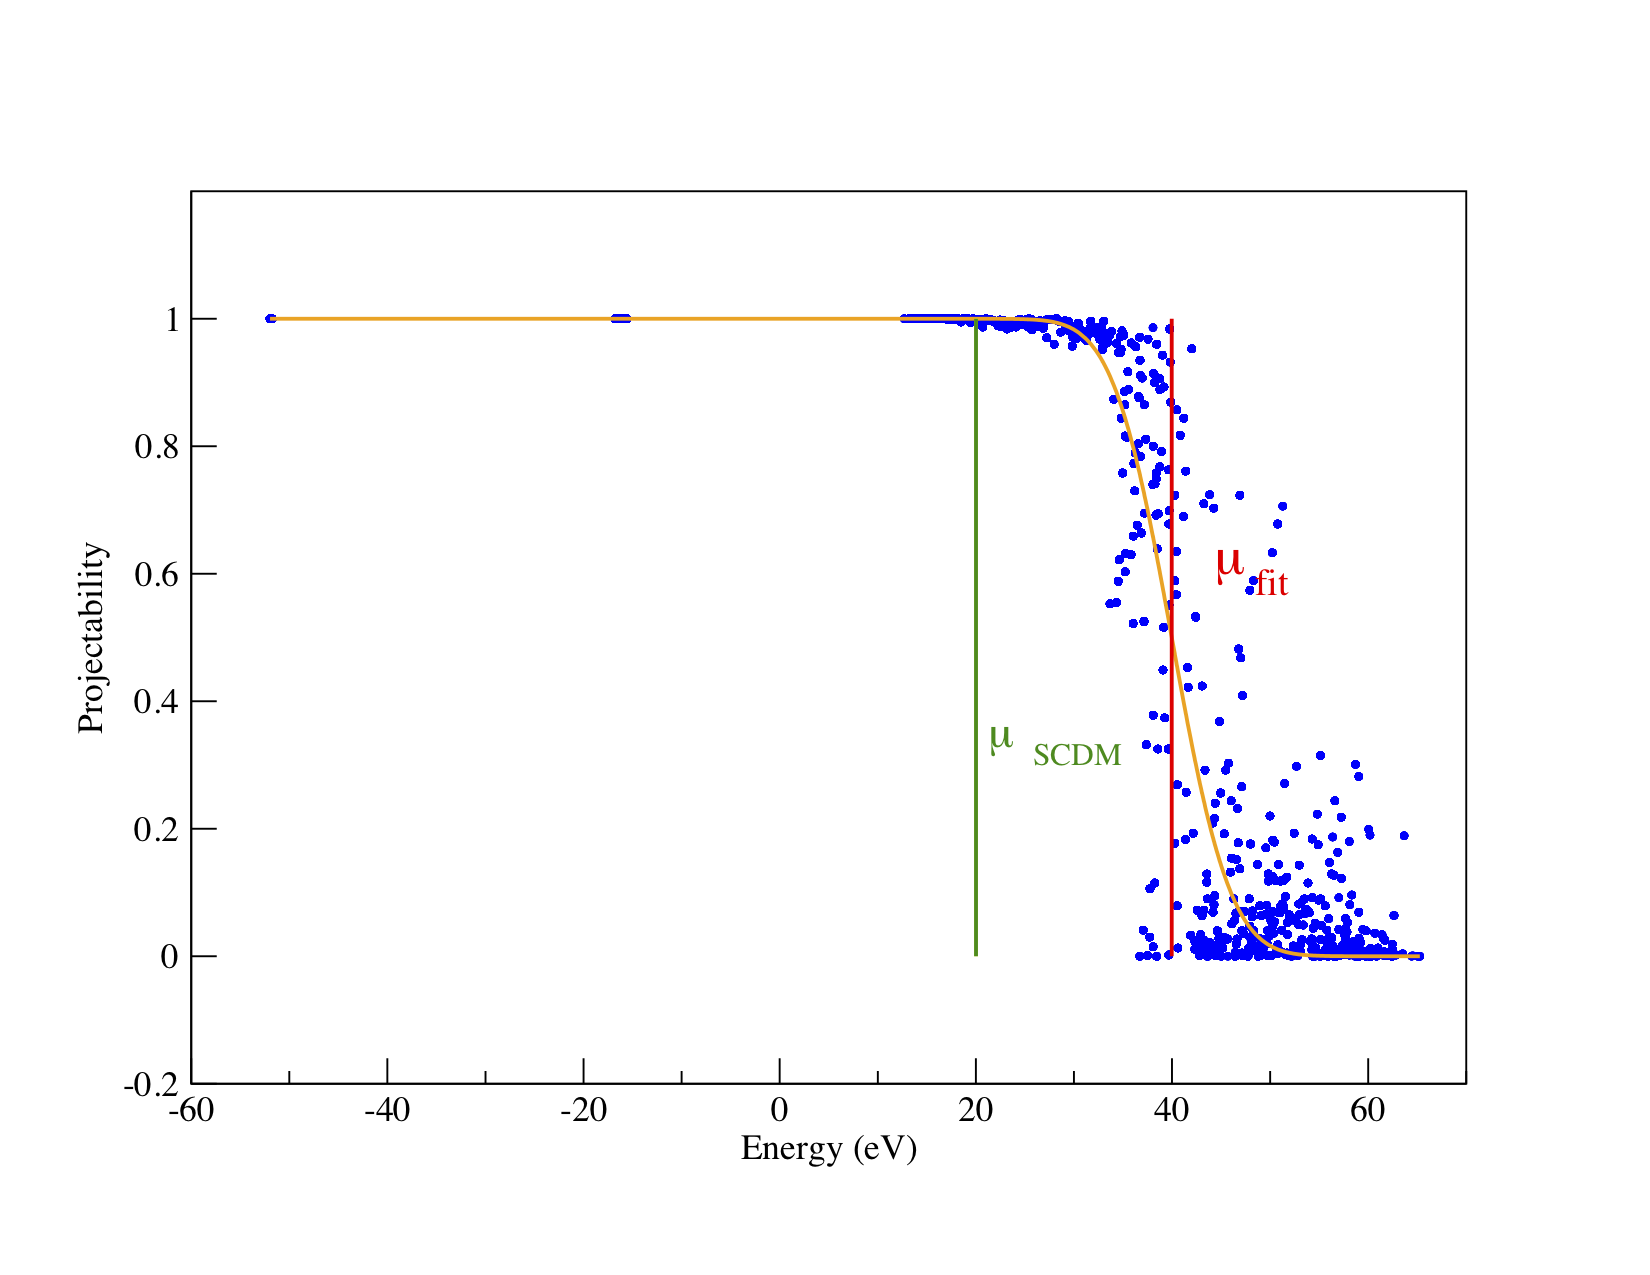
\includegraphics[width=0.45\columnwidth]{./W_fit.png}}
\subfloat[]{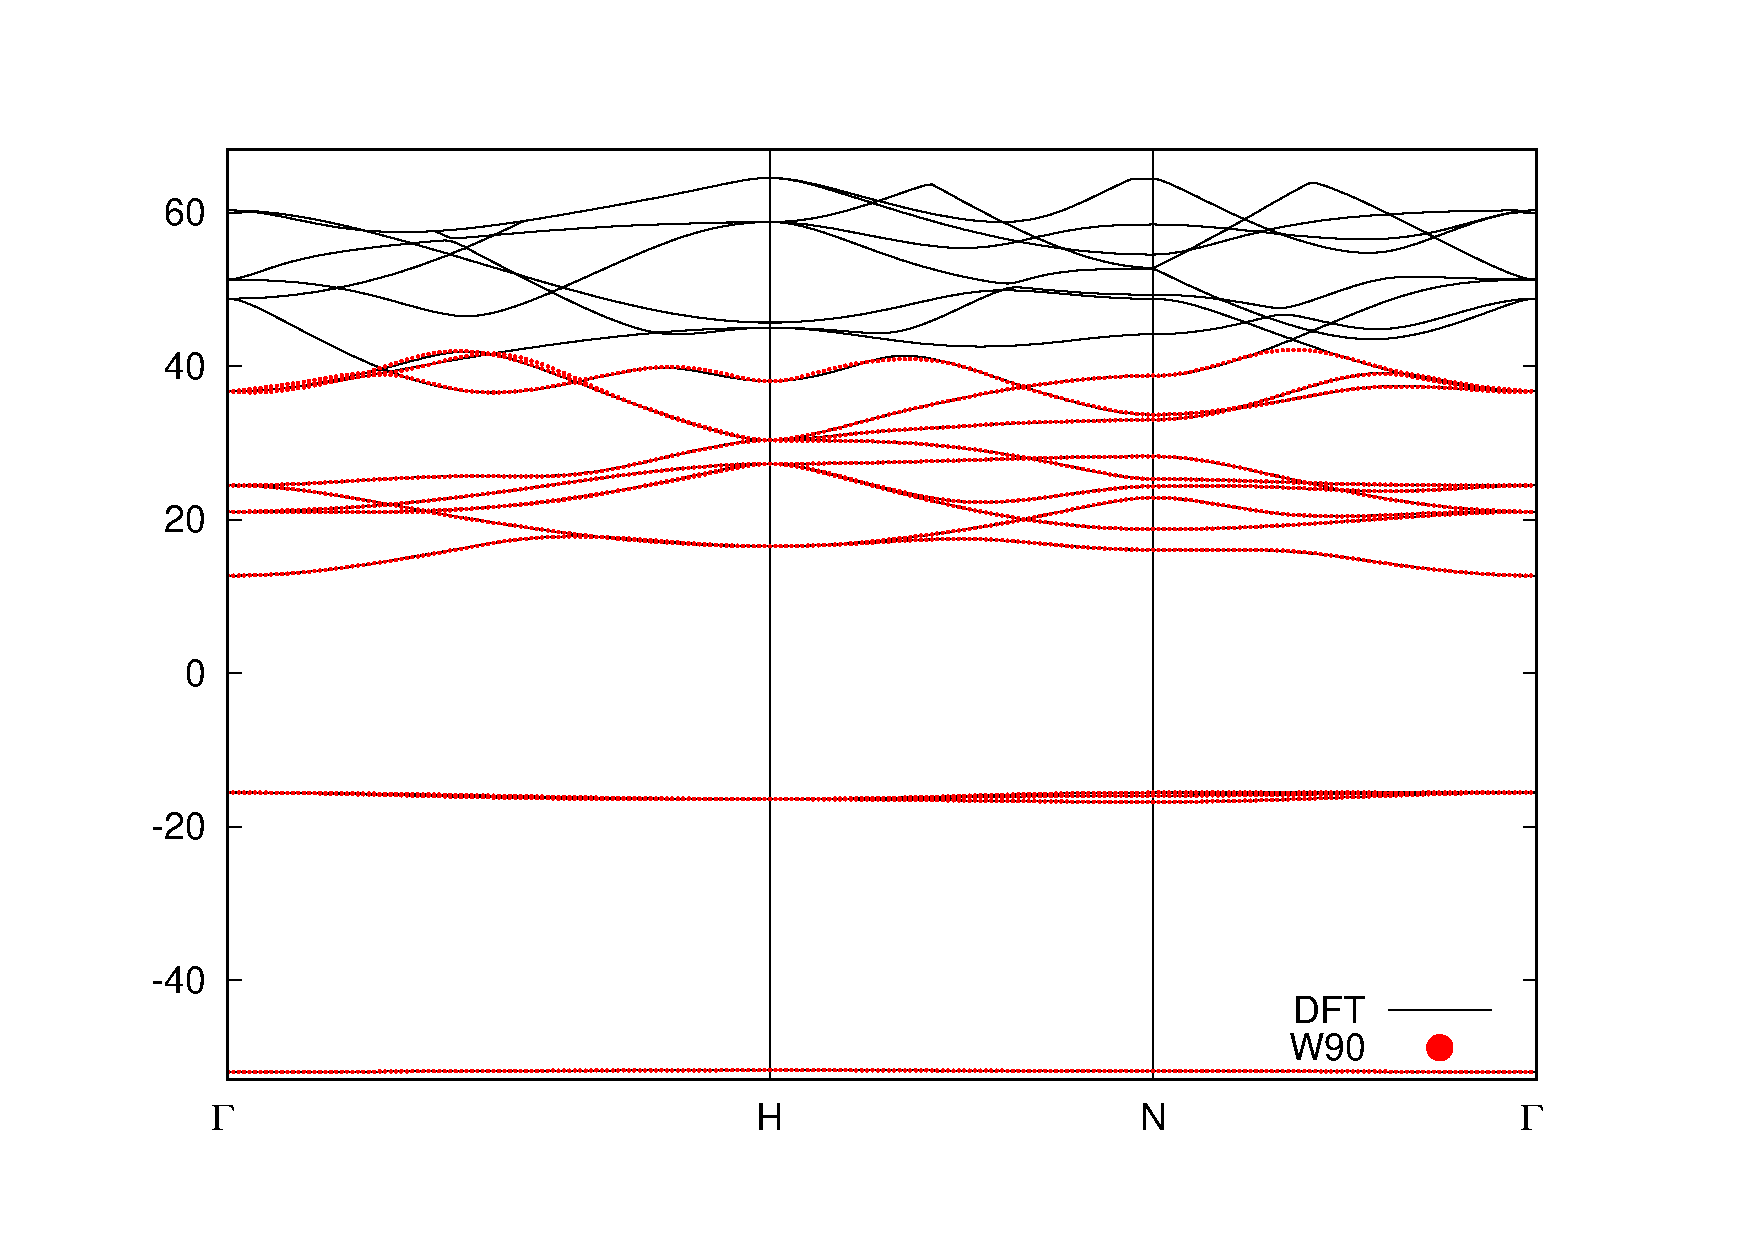
\includegraphics[width=0.45\columnwidth]{./W_bs.pdf}}
\caption{ a) Each blue dot represents the projectability as defined in Eq. (22) of Ref. \cite{Vitale2019automated}  of the state
$\vert n\mathbf{k} \rangle$ as a function of the corresponding energy $\epsilon_{n\mathbf{k}}$ for tungsten. The yellow line shows the fitted complementary error function. The vertical red line represents the value of $\sigma_{fit}$ while the vertical green line represents the optimal value of $\mu_{SCDM}$, i.e. $\mu_{SCDM} = \mu_{fit} - 3\sigma_{fit}$. b) Band structure of tungsten on the $\Gamma$-H-N-$\Gamma$ path from DFT calculations (solid black) and Wannier interpolation using the SCDM method to construct the initial guess (red dots).}
\label{fig:W_fit}
\end{figure}

%\cleardoublepage

\bibliographystyle{apsrev4-1}
\bibliography{../wannier90}

\end{document}
